\documentclass[twoside]{book}

% Packages required by doxygen
\usepackage{calc}
\usepackage{doxygen}
\usepackage{graphicx}
\usepackage[utf8]{inputenc}
\usepackage{makeidx}
\usepackage{multicol}
\usepackage{multirow}
\usepackage{textcomp}
\usepackage[table]{xcolor}

% Font selection
\usepackage[T1]{fontenc}
\usepackage{mathptmx}
\usepackage[scaled=.90]{helvet}
\usepackage{courier}
\usepackage{amssymb}
\usepackage{sectsty}
\renewcommand{\familydefault}{\sfdefault}
\allsectionsfont{%
  \fontseries{bc}\selectfont%
  \color{darkgray}%
}
\renewcommand{\DoxyLabelFont}{%
  \fontseries{bc}\selectfont%
  \color{darkgray}%
}

% Page & text layout
\usepackage{geometry}
\geometry{%
  a4paper,%
  top=2.5cm,%
  bottom=2.5cm,%
  left=2.5cm,%
  right=2.5cm%
}
\tolerance=750
\hfuzz=15pt
\hbadness=750
\setlength{\emergencystretch}{15pt}
\setlength{\parindent}{0cm}
\setlength{\parskip}{0.2cm}
\makeatletter
\renewcommand{\paragraph}{%
  \@startsection{paragraph}{4}{0ex}{-1.0ex}{1.0ex}{%
    \normalfont\normalsize\bfseries\SS@parafont%
  }%
}
\renewcommand{\subparagraph}{%
  \@startsection{subparagraph}{5}{0ex}{-1.0ex}{1.0ex}{%
    \normalfont\normalsize\bfseries\SS@subparafont%
  }%
}
\makeatother

% Headers & footers
\usepackage{fancyhdr}
\pagestyle{fancyplain}
\fancyhead[LE]{\fancyplain{}{\bfseries\thepage}}
\fancyhead[CE]{\fancyplain{}{}}
\fancyhead[RE]{\fancyplain{}{\bfseries\leftmark}}
\fancyhead[LO]{\fancyplain{}{\bfseries\rightmark}}
\fancyhead[CO]{\fancyplain{}{}}
\fancyhead[RO]{\fancyplain{}{\bfseries\thepage}}
\fancyfoot[LE]{\fancyplain{}{}}
\fancyfoot[CE]{\fancyplain{}{}}
\fancyfoot[RE]{\fancyplain{}{\bfseries\scriptsize Generated on Mon Dec 30 2013 11\-:02\-:23 for Single Cycled Simple Risc Processor Design in V\-H\-D\-L by Doxygen }}
\fancyfoot[LO]{\fancyplain{}{\bfseries\scriptsize Generated on Mon Dec 30 2013 11\-:02\-:23 for Single Cycled Simple Risc Processor Design in V\-H\-D\-L by Doxygen }}
\fancyfoot[CO]{\fancyplain{}{}}
\fancyfoot[RO]{\fancyplain{}{}}
\renewcommand{\footrulewidth}{0.4pt}
\renewcommand{\chaptermark}[1]{%
  \markboth{#1}{}%
}
\renewcommand{\sectionmark}[1]{%
  \markright{\thesection\ #1}%
}

% Indices & bibliography
\usepackage{natbib}
\usepackage[titles]{tocloft}
\setcounter{tocdepth}{3}
\setcounter{secnumdepth}{5}
\makeindex

% Hyperlinks (required, but should be loaded last)
\usepackage{ifpdf}
\ifpdf
  \usepackage[pdftex,pagebackref=true]{hyperref}
\else
  \usepackage[ps2pdf,pagebackref=true]{hyperref}
\fi
\hypersetup{%
  colorlinks=true,%
  linkcolor=blue,%
  citecolor=blue,%
  unicode%
}

% Custom commands
\newcommand{\clearemptydoublepage}{%
  \newpage{\pagestyle{empty}\cleardoublepage}%
}


%===== C O N T E N T S =====

\begin{document}

% Titlepage & ToC
\hypersetup{pageanchor=false}
\pagenumbering{roman}
\begin{titlepage}
\vspace*{7cm}
\begin{center}%
{\Large Single Cycled Simple Risc Processor Design in V\-H\-D\-L }\\
\vspace*{1cm}
{\large Generated by Doxygen 1.8.5}\\
\vspace*{0.5cm}
{\small Mon Dec 30 2013 11:02:23}\\
\end{center}
\end{titlepage}
\clearemptydoublepage
\tableofcontents
\clearemptydoublepage
\pagenumbering{arabic}
\hypersetup{pageanchor=true}

%--- Begin generated contents ---
\chapter{Namespace Index}
\section{Packages}
Here are the packages with brief descriptions (if available)\-:\begin{DoxyCompactList}
\item\contentsline{section}{\hyperlink{classfile_read}{file\-Read} \\*This function converts a char to std\-\_\-logic }{\pageref{namespacefile_read}}{}
\end{DoxyCompactList}

\chapter{Design Unit Index}
\section{Design Unit Hierarchy}
This inheritance list is sorted roughly, but not completely, alphabetically\-:\begin{DoxyCompactList}
\item \contentsline{section}{Simple\-R\-I\-S\-C}{\pageref{class_simple_r_i_s_c}}{}
\begin{DoxyCompactList}
\item \contentsline{section}{I\-F\-Unit}{\pageref{class_i_f_unit}}{}
\item \contentsline{section}{C\-Unit}{\pageref{class_c_unit}}{}
\item \contentsline{section}{O\-F\-Unit}{\pageref{class_o_f_unit}}{}
\item \contentsline{section}{E\-X\-Unit}{\pageref{class_e_x_unit}}{}
\item \contentsline{section}{M\-A\-Unit}{\pageref{class_m_a_unit}}{}
\end{DoxyCompactList}
\end{DoxyCompactList}

\chapter{Design Unit Index}
\section{Design Unit List}
Here is a list of all design unit members with links to the Entities they belong to\-:\begin{DoxyCompactList}
\item\contentsline{section}{architecture \hyperlink{class_e_x_unit_1_1_a_l_u___b_u}{A\-L\-U\-\_\-\-B\-U} \\*O\-F\-U is the architectural description of the E\-X Unit }{\pageref{class_e_x_unit_1_1_a_l_u___b_u}}{}
\item\contentsline{section}{architecture \hyperlink{class_c_unit_1_1_c_u}{C\-U} \\*\hyperlink{class_c_unit_1_1_c_u}{C\-U} is the architectural description of the Control Unit }{\pageref{class_c_unit_1_1_c_u}}{}
\item\contentsline{section}{entity \hyperlink{class_c_unit}{C\-Unit} \\*This is the unit that generates the control signals }{\pageref{class_c_unit}}{}
\item\contentsline{section}{architecture \hyperlink{class_m_a_unit_1_1_d_m}{D\-M} \\*\hyperlink{class_m_a_unit_1_1_d_m}{D\-M} is the architecture of the Memory Unit }{\pageref{class_m_a_unit_1_1_d_m}}{}
\item\contentsline{section}{entity \hyperlink{class_e_x_unit}{E\-X\-Unit} \\*This is the unit that implements the A\-L\-U and branch Unit }{\pageref{class_e_x_unit}}{}
\item\contentsline{section}{entity \hyperlink{class_i_f_unit}{I\-F\-Unit} \\*This is the unit that implements the Instruction fetch Unit }{\pageref{class_i_f_unit}}{}
\item\contentsline{section}{architecture \hyperlink{class_i_f_unit_1_1_i_m}{I\-M} \\*\hyperlink{class_i_f_unit_1_1_i_m}{I\-M} is the architectural description of the Instruction Fetch Unit }{\pageref{class_i_f_unit_1_1_i_m}}{}
\item\contentsline{section}{architecture \hyperlink{class_simple_r_i_s_c_1_1main}{main} }{\pageref{class_simple_r_i_s_c_1_1main}}{}
\item\contentsline{section}{entity \hyperlink{class_m_a_unit}{M\-A\-Unit} \\*This is the unit that implements a R\-A\-M }{\pageref{class_m_a_unit}}{}
\item\contentsline{section}{architecture \hyperlink{class_o_f_unit_1_1_o_f_u}{O\-F\-U} \\*\hyperlink{class_o_f_unit_1_1_o_f_u}{O\-F\-U} is the architectural description of the operand fetch unit and register file }{\pageref{class_o_f_unit_1_1_o_f_u}}{}
\item\contentsline{section}{entity \hyperlink{class_o_f_unit}{O\-F\-Unit} \\*This the Operand Fetch Unit which also contains the register file implementation }{\pageref{class_o_f_unit}}{}
\item\contentsline{section}{entity \hyperlink{class_simple_r_i_s_c}{Simple\-R\-I\-S\-C} \\*This is empty shell for the main compilation of all the other components in the processor }{\pageref{class_simple_r_i_s_c}}{}
\end{DoxyCompactList}

\chapter{File Index}
\section{File List}
Here is a list of all documented files with brief descriptions\-:\begin{DoxyCompactList}
\item\contentsline{section}{\hyperlink{_c_unit_8vhdl}{C\-Unit.\-vhdl} \\*This file for the implementation of a Control Unit for the processor }{\pageref{_c_unit_8vhdl}}{}
\item\contentsline{section}{\hyperlink{_e_x_unit_8vhdl}{E\-X\-Unit.\-vhdl} \\*This file is for the Arithmetic and logic Unit of the processor }{\pageref{_e_x_unit_8vhdl}}{}
\item\contentsline{section}{\hyperlink{file_read_8vhdl}{file\-Read.\-vhdl} \\*This file for the implementation of file reading function }{\pageref{file_read_8vhdl}}{}
\item\contentsline{section}{\hyperlink{_i_f_unit_8vhdl}{I\-F\-Unit.\-vhdl} \\*This file for the implementation of a Instruction Fetch Unit for the processor }{\pageref{_i_f_unit_8vhdl}}{}
\item\contentsline{section}{\hyperlink{_m_a_unit_8vhdl}{M\-A\-Unit.\-vhdl} \\*This file for the implementation of a memory for the processor }{\pageref{_m_a_unit_8vhdl}}{}
\item\contentsline{section}{\hyperlink{_o_f_unit_8vhdl}{O\-F\-Unit.\-vhdl} \\*Operand Fetch unit as well as register read and write operations implemented }{\pageref{_o_f_unit_8vhdl}}{}
\item\contentsline{section}{\hyperlink{_simple_r_i_s_c_8vhdl}{Simple\-R\-I\-S\-C.\-vhdl} \\*This is compilation of all the components of the processor }{\pageref{_simple_r_i_s_c_8vhdl}}{}
\end{DoxyCompactList}

\chapter{Namespace Documentation}
\hypertarget{namespacefile_read}{\section{file\-Read Namespace Reference}
\label{namespacefile_read}\index{file\-Read@{file\-Read}}
}


This function converts a char to std\-\_\-logic.  




\subsection{Detailed Description}
This function converts a char to std\-\_\-logic. 
\chapter{Class Documentation}
\hypertarget{class__file_read}{\section{file\-Read Package Body Reference}
\label{class__file_read}\index{file\-Read@{file\-Read}}
}
{\bfseries Package $>$$>$ }\hyperlink{classfile_read}{file\-Read}\\*
\subsection*{Functions}
 \begin{DoxyCompactItemize}
\item 
\hypertarget{class__file_read_a130c40cc008de8d3ccb7e18201a712b9}{{\bfseries {\bfseries \textcolor{comment}{std\-\_\-logic}\textcolor{vhdlchar}{ }}} \hyperlink{class__file_read_a130c40cc008de8d3ccb7e18201a712b9}{to\-\_\-std\-\_\-logic\-\_\-from\-\_\-char}{\bfseries  ( }{\bfseries \textcolor{vhdlchar}{data\-: }\textcolor{stringliteral}{in }{\bfseries \textcolor{comment}{character}\textcolor{vhdlchar}{ }}}{\bfseries  )} }\label{class__file_read_a130c40cc008de8d3ccb7e18201a712b9}

\item 
\hypertarget{class__file_read_a2f37cc7e400e439a39996222cc6c4773}{{\bfseries {\bfseries \textcolor{comment}{std\-\_\-logic\-\_\-vector}\textcolor{vhdlchar}{ }}} \hyperlink{class__file_read_a2f37cc7e400e439a39996222cc6c4773}{to\-\_\-std\-\_\-logic\-\_\-vector}{\bfseries  ( }{\bfseries \textcolor{vhdlchar}{data\-: }\textcolor{stringliteral}{in }{\bfseries \textcolor{comment}{string}\textcolor{vhdlchar}{ }}}{\bfseries  )} }\label{class__file_read_a2f37cc7e400e439a39996222cc6c4773}

\end{DoxyCompactItemize}


The documentation for this class was generated from the following file\-:\begin{DoxyCompactItemize}
\item 
\hyperlink{file_read_8vhdl}{file\-Read.\-vhdl}\end{DoxyCompactItemize}

\hypertarget{class_e_x_unit_1_1_a_l_u___b_u}{\section{A\-L\-U\-\_\-\-B\-U Architecture Reference}
\label{class_e_x_unit_1_1_a_l_u___b_u}\index{A\-L\-U\-\_\-\-B\-U@{A\-L\-U\-\_\-\-B\-U}}
}


O\-F\-U is the architectural description of the E\-X Unit.  


\subsection*{Signals}
 \begin{DoxyCompactItemize}
\item 
\hypertarget{class_e_x_unit_1_1_a_l_u___b_u_abb079547a7e3a2edc783079e496ab230}{\hyperlink{class_e_x_unit_1_1_a_l_u___b_u_abb079547a7e3a2edc783079e496ab230}{E} {\bfseries \textcolor{comment}{boolean}\textcolor{vhdlchar}{ }\textcolor{vhdlchar}{ }\textcolor{vhdlchar}{\-:}\textcolor{vhdlchar}{=}\textcolor{vhdlchar}{ }\textcolor{vhdlchar}{false}\textcolor{vhdlchar}{ }} }\label{class_e_x_unit_1_1_a_l_u___b_u_abb079547a7e3a2edc783079e496ab230}

\begin{DoxyCompactList}\small\item\em a boolean signal storing the boolean value of equality operation \end{DoxyCompactList}\item 
\hypertarget{class_e_x_unit_1_1_a_l_u___b_u_a11b1a9c5106ad3b13e91ab299fe53ffc}{\hyperlink{class_e_x_unit_1_1_a_l_u___b_u_a11b1a9c5106ad3b13e91ab299fe53ffc}{G\-T} {\bfseries \textcolor{comment}{boolean}\textcolor{vhdlchar}{ }\textcolor{vhdlchar}{ }\textcolor{vhdlchar}{\-:}\textcolor{vhdlchar}{=}\textcolor{vhdlchar}{ }\textcolor{vhdlchar}{false}\textcolor{vhdlchar}{ }} }\label{class_e_x_unit_1_1_a_l_u___b_u_a11b1a9c5106ad3b13e91ab299fe53ffc}

\begin{DoxyCompactList}\small\item\em a boolean signal storing the boolean value of greater-\/than operation \end{DoxyCompactList}\item 
\hypertarget{class_e_x_unit_1_1_a_l_u___b_u_abd1839792ee9767d875129a826b25303}{\hyperlink{class_e_x_unit_1_1_a_l_u___b_u_abd1839792ee9767d875129a826b25303}{A} {\bfseries \textcolor{comment}{std\-\_\-logic\-\_\-vector}\textcolor{vhdlchar}{ }\textcolor{vhdlchar}{(}\textcolor{vhdlchar}{ } \textcolor{vhdldigit}{31} \textcolor{vhdlchar}{ }\textcolor{vhdlchar}{ }\textcolor{vhdlchar}{ }\textcolor{vhdlkeyword}{downto}\textcolor{vhdlchar}{ }\textcolor{vhdlchar}{ }\textcolor{vhdlchar}{ } \textcolor{vhdldigit}{0} \textcolor{vhdlchar}{ }\textcolor{vhdlchar}{)}\textcolor{vhdlchar}{ }} }\label{class_e_x_unit_1_1_a_l_u___b_u_abd1839792ee9767d875129a826b25303}

\begin{DoxyCompactList}\small\item\em The first operand in the A\-L\-U. \end{DoxyCompactList}\item 
\hypertarget{class_e_x_unit_1_1_a_l_u___b_u_a5994cf9514855203a6cb1fa380cc53db}{\hyperlink{class_e_x_unit_1_1_a_l_u___b_u_a5994cf9514855203a6cb1fa380cc53db}{B} {\bfseries \textcolor{comment}{std\-\_\-logic\-\_\-vector}\textcolor{vhdlchar}{ }\textcolor{vhdlchar}{(}\textcolor{vhdlchar}{ } \textcolor{vhdldigit}{31} \textcolor{vhdlchar}{ }\textcolor{vhdlchar}{ }\textcolor{vhdlchar}{ }\textcolor{vhdlkeyword}{downto}\textcolor{vhdlchar}{ }\textcolor{vhdlchar}{ }\textcolor{vhdlchar}{ } \textcolor{vhdldigit}{0} \textcolor{vhdlchar}{ }\textcolor{vhdlchar}{)}\textcolor{vhdlchar}{ }} }\label{class_e_x_unit_1_1_a_l_u___b_u_a5994cf9514855203a6cb1fa380cc53db}

\begin{DoxyCompactList}\small\item\em The second operand in the A\-L\-U. \end{DoxyCompactList}\end{DoxyCompactItemize}


\subsection{Detailed Description}
O\-F\-U is the architectural description of the E\-X Unit. 

The documentation for this class was generated from the following file\-:\begin{DoxyCompactItemize}
\item 
\hyperlink{_e_x_unit_8vhdl}{E\-X\-Unit.\-vhdl}\end{DoxyCompactItemize}

\hypertarget{class_c_unit_1_1_c_u}{\section{C\-U Architecture Reference}
\label{class_c_unit_1_1_c_u}\index{C\-U@{C\-U}}
}


\hyperlink{class_c_unit_1_1_c_u}{C\-U} is the architectural description of the Control Unit.  


\subsection*{Processes}
 \begin{DoxyCompactItemize}
\item 
\hypertarget{class_c_unit_1_1_c_u_a14098fa528925c40a4e31e81a5783afa}{\hyperlink{class_c_unit_1_1_c_u_a14098fa528925c40a4e31e81a5783afa}{P\-R\-O\-C\-E\-S\-S\-\_\-0}{\bfseries  ( {\bfseries {\bfseries \hyperlink{class_c_unit_1_1_c_u_a6f3dbf2da02fe7917066d92bf3f32032}{op\-\_\-code}} \textcolor{vhdlchar}{ }\textcolor{vhdlchar}{ }\textcolor{vhdlchar}{ }} , {\bfseries {\bfseries \hyperlink{class_c_unit_1_1_c_u_acc0e964d67e878c4c363942b522e297c}{I}} \textcolor{vhdlchar}{ }} )}}\label{class_c_unit_1_1_c_u_a14098fa528925c40a4e31e81a5783afa}

\begin{DoxyCompactList}\small\item\em Extracting the opcode from the 32-\/bit instruction. \end{DoxyCompactList}\end{DoxyCompactItemize}
\subsection*{Signals}
 \begin{DoxyCompactItemize}
\item 
\hypertarget{class_c_unit_1_1_c_u_a6f3dbf2da02fe7917066d92bf3f32032}{\hyperlink{class_c_unit_1_1_c_u_a6f3dbf2da02fe7917066d92bf3f32032}{op\-\_\-code} {\bfseries \textcolor{comment}{std\-\_\-logic\-\_\-vector}\textcolor{vhdlchar}{ }\textcolor{vhdlchar}{(}\textcolor{vhdlchar}{ } \textcolor{vhdldigit}{4} \textcolor{vhdlchar}{ }\textcolor{vhdlchar}{ }\textcolor{vhdlchar}{ }\textcolor{vhdlkeyword}{downto}\textcolor{vhdlchar}{ }\textcolor{vhdlchar}{ }\textcolor{vhdlchar}{ } \textcolor{vhdldigit}{0} \textcolor{vhdlchar}{ }\textcolor{vhdlchar}{)}\textcolor{vhdlchar}{ }} }\label{class_c_unit_1_1_c_u_a6f3dbf2da02fe7917066d92bf3f32032}

\begin{DoxyCompactList}\small\item\em A vector containing 5 bits of the instruction marking the instruction type. \end{DoxyCompactList}\item 
\hypertarget{class_c_unit_1_1_c_u_acc0e964d67e878c4c363942b522e297c}{\hyperlink{class_c_unit_1_1_c_u_acc0e964d67e878c4c363942b522e297c}{I} {\bfseries \textcolor{comment}{std\-\_\-logic}\textcolor{vhdlchar}{ }} }\label{class_c_unit_1_1_c_u_acc0e964d67e878c4c363942b522e297c}

\begin{DoxyCompactList}\small\item\em The immediate bit. \end{DoxyCompactList}\end{DoxyCompactItemize}


\subsection{Detailed Description}
\hyperlink{class_c_unit_1_1_c_u}{C\-U} is the architectural description of the Control Unit. 

The documentation for this class was generated from the following file\-:\begin{DoxyCompactItemize}
\item 
\hyperlink{_c_unit_8vhdl}{C\-Unit.\-vhdl}\end{DoxyCompactItemize}

\hypertarget{class_c_unit}{\section{C\-Unit Entity Reference}
\label{class_c_unit}\index{C\-Unit@{C\-Unit}}
}


This is the unit that generates the control signals.  


Inheritance diagram for C\-Unit\-:\begin{figure}[H]
\begin{center}
\leavevmode
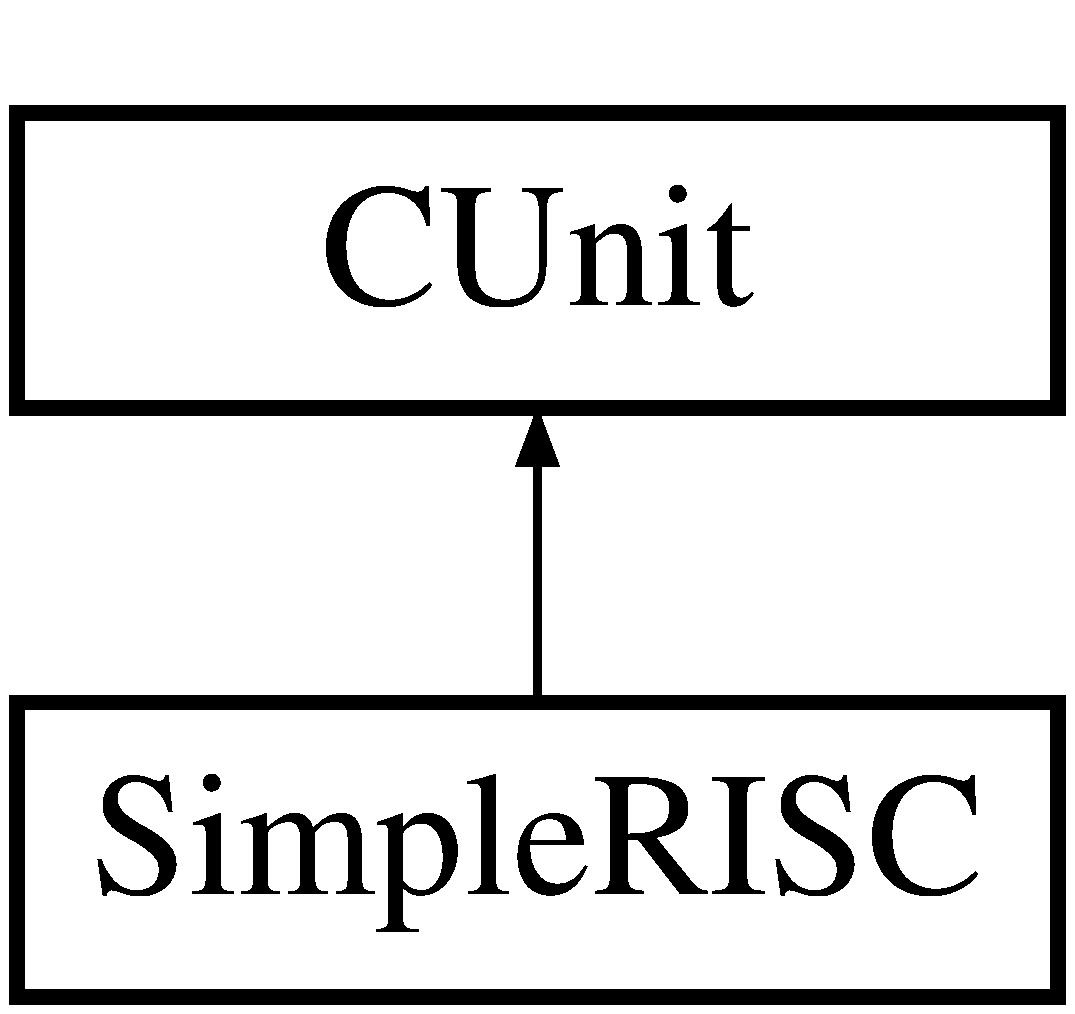
\includegraphics[height=2.000000cm]{class_c_unit}
\end{center}
\end{figure}
\subsection*{Entities}
\begin{DoxyCompactItemize}
\item 
\hyperlink{class_c_unit_1_1_c_u}{C\-U} architecture
\begin{DoxyCompactList}\small\item\em \hyperlink{class_c_unit_1_1_c_u}{C\-U} is the architectural description of the Control Unit. \end{DoxyCompactList}\end{DoxyCompactItemize}
\subsection*{Libraries}
 \begin{DoxyCompactItemize}
\item 
\hypertarget{class_c_unit_a0a6af6eef40212dbaf130d57ce711256}{\hyperlink{class_c_unit_a0a6af6eef40212dbaf130d57ce711256}{ieee} }\label{class_c_unit_a0a6af6eef40212dbaf130d57ce711256}

\end{DoxyCompactItemize}
\subsection*{Use Clauses}
 \begin{DoxyCompactItemize}
\item 
\hypertarget{class_c_unit_a43ecb358105806229eb7a3074fc4d577}{\hyperlink{class_c_unit_a43ecb358105806229eb7a3074fc4d577}{ieee.\-std\-\_\-logic\-\_\-1164.\-all}   }\label{class_c_unit_a43ecb358105806229eb7a3074fc4d577}

\end{DoxyCompactItemize}
\subsection*{Ports}
 \begin{DoxyCompactItemize}
\item 
\hypertarget{class_c_unit_a187326d2b4b17c46dcaeead2064c8c82}{\hyperlink{class_c_unit_a187326d2b4b17c46dcaeead2064c8c82}{Instruction}  {\bfseries {\bfseries \textcolor{vhdlkeyword}{in}\textcolor{vhdlchar}{ }}} {\bfseries \textcolor{comment}{std\-\_\-logic\-\_\-vector}\textcolor{vhdlchar}{ }\textcolor{vhdlchar}{(}\textcolor{vhdlchar}{ } \textcolor{vhdldigit}{31} \textcolor{vhdlchar}{ }\textcolor{vhdlchar}{ }\textcolor{vhdlchar}{ }\textcolor{vhdlkeyword}{downto}\textcolor{vhdlchar}{ }\textcolor{vhdlchar}{ }\textcolor{vhdlchar}{ } \textcolor{vhdldigit}{0} \textcolor{vhdlchar}{ }\textcolor{vhdlchar}{)}\textcolor{vhdlchar}{ }} }\label{class_c_unit_a187326d2b4b17c46dcaeead2064c8c82}

\begin{DoxyCompactList}\small\item\em The 32-\/bit instruction coming from the Instruction fetch Unit. \end{DoxyCompactList}\item 
\hypertarget{class_c_unit_a81134d903eb6d6b92bfee5560162a63a}{\hyperlink{class_c_unit_a81134d903eb6d6b92bfee5560162a63a}{is\-Mov}  {\bfseries {\bfseries \textcolor{vhdlkeyword}{out}\textcolor{vhdlchar}{ }}} {\bfseries \textcolor{comment}{boolean}\textcolor{vhdlchar}{ }} }\label{class_c_unit_a81134d903eb6d6b92bfee5560162a63a}

\begin{DoxyCompactList}\small\item\em boolean which states whether the instruction is 'mov' \end{DoxyCompactList}\item 
\hypertarget{class_c_unit_acf493c1820670da4fa6e856436fae09c}{\hyperlink{class_c_unit_acf493c1820670da4fa6e856436fae09c}{is\-St}  {\bfseries {\bfseries \textcolor{vhdlkeyword}{out}\textcolor{vhdlchar}{ }}} {\bfseries \textcolor{comment}{boolean}\textcolor{vhdlchar}{ }} }\label{class_c_unit_acf493c1820670da4fa6e856436fae09c}

\begin{DoxyCompactList}\small\item\em boolean which states whether the instruction is 'st' \end{DoxyCompactList}\item 
\hypertarget{class_c_unit_ad35c473f9f330123d545e49e48459bec}{\hyperlink{class_c_unit_ad35c473f9f330123d545e49e48459bec}{is\-Ld}  {\bfseries {\bfseries \textcolor{vhdlkeyword}{out}\textcolor{vhdlchar}{ }}} {\bfseries \textcolor{comment}{boolean}\textcolor{vhdlchar}{ }} }\label{class_c_unit_ad35c473f9f330123d545e49e48459bec}

\begin{DoxyCompactList}\small\item\em boolean which states whether the instruction is 'ld' \end{DoxyCompactList}\item 
\hypertarget{class_c_unit_aebbb21b47d7fdc5172ad6c088a2c339b}{\hyperlink{class_c_unit_aebbb21b47d7fdc5172ad6c088a2c339b}{is\-Beq}  {\bfseries {\bfseries \textcolor{vhdlkeyword}{out}\textcolor{vhdlchar}{ }}} {\bfseries \textcolor{comment}{boolean}\textcolor{vhdlchar}{ }} }\label{class_c_unit_aebbb21b47d7fdc5172ad6c088a2c339b}

\begin{DoxyCompactList}\small\item\em boolean which states whether the instruction is 'beq' \end{DoxyCompactList}\item 
\hypertarget{class_c_unit_a1df57aa5d86b9d2c21f1ca79aacac3f9}{\hyperlink{class_c_unit_a1df57aa5d86b9d2c21f1ca79aacac3f9}{is\-Bgt}  {\bfseries {\bfseries \textcolor{vhdlkeyword}{out}\textcolor{vhdlchar}{ }}} {\bfseries \textcolor{comment}{boolean}\textcolor{vhdlchar}{ }} }\label{class_c_unit_a1df57aa5d86b9d2c21f1ca79aacac3f9}

\begin{DoxyCompactList}\small\item\em boolean which states whether the instruction is 'bgt' \end{DoxyCompactList}\item 
\hypertarget{class_c_unit_a98e2b65456db66badf1296ad798288be}{\hyperlink{class_c_unit_a98e2b65456db66badf1296ad798288be}{is\-Immediate}  {\bfseries {\bfseries \textcolor{vhdlkeyword}{out}\textcolor{vhdlchar}{ }}} {\bfseries \textcolor{comment}{boolean}\textcolor{vhdlchar}{ }} }\label{class_c_unit_a98e2b65456db66badf1296ad798288be}

\begin{DoxyCompactList}\small\item\em boolean which the instruction has an immediate as the arguments. \end{DoxyCompactList}\item 
\hypertarget{class_c_unit_ab8f0ec8ea90e74b7d464ecad474f9c67}{\hyperlink{class_c_unit_ab8f0ec8ea90e74b7d464ecad474f9c67}{is\-Wb}  {\bfseries {\bfseries \textcolor{vhdlkeyword}{out}\textcolor{vhdlchar}{ }}} {\bfseries \textcolor{comment}{boolean}\textcolor{vhdlchar}{ }} }\label{class_c_unit_ab8f0ec8ea90e74b7d464ecad474f9c67}

\begin{DoxyCompactList}\small\item\em boolean whether something has to be written into the register file. \end{DoxyCompactList}\item 
\hypertarget{class_c_unit_ac34d5f9af81ab3e2e3aa51f7c1e267b3}{\hyperlink{class_c_unit_ac34d5f9af81ab3e2e3aa51f7c1e267b3}{is\-U\-Branch}  {\bfseries {\bfseries \textcolor{vhdlkeyword}{out}\textcolor{vhdlchar}{ }}} {\bfseries \textcolor{comment}{boolean}\textcolor{vhdlchar}{ }} }\label{class_c_unit_ac34d5f9af81ab3e2e3aa51f7c1e267b3}

\begin{DoxyCompactList}\small\item\em boolean whether the statement is a direct branching one(b, ret, call) \end{DoxyCompactList}\item 
\hypertarget{class_c_unit_acd79f46efcd273deffa5a712e1d155b3}{\hyperlink{class_c_unit_acd79f46efcd273deffa5a712e1d155b3}{is\-Ret}  {\bfseries {\bfseries \textcolor{vhdlkeyword}{out}\textcolor{vhdlchar}{ }}} {\bfseries \textcolor{comment}{boolean}\textcolor{vhdlchar}{ }} }\label{class_c_unit_acd79f46efcd273deffa5a712e1d155b3}

\begin{DoxyCompactList}\small\item\em boolean which states whether the instruction is 'ret' \end{DoxyCompactList}\item 
\hypertarget{class_c_unit_a455d189bc702a8327ce22986cbf13c49}{\hyperlink{class_c_unit_a455d189bc702a8327ce22986cbf13c49}{is\-Call}  {\bfseries {\bfseries \textcolor{vhdlkeyword}{out}\textcolor{vhdlchar}{ }}} {\bfseries \textcolor{comment}{boolean}\textcolor{vhdlchar}{ }} }\label{class_c_unit_a455d189bc702a8327ce22986cbf13c49}

\begin{DoxyCompactList}\small\item\em boolean which states whether the instruction is 'call' \end{DoxyCompactList}\item 
\hypertarget{class_c_unit_a871a1f390d61fb699f64ca9a3f332772}{\hyperlink{class_c_unit_a871a1f390d61fb699f64ca9a3f332772}{alu\-S}  {\bfseries {\bfseries \textcolor{vhdlkeyword}{out}\textcolor{vhdlchar}{ }}} {\bfseries \textcolor{comment}{std\-\_\-logic\-\_\-vector}\textcolor{vhdlchar}{ }\textcolor{vhdlchar}{(}\textcolor{vhdlchar}{ } \textcolor{vhdldigit}{2} \textcolor{vhdlchar}{ }\textcolor{vhdlchar}{ }\textcolor{vhdlchar}{ }\textcolor{vhdlkeyword}{downto}\textcolor{vhdlchar}{ }\textcolor{vhdlchar}{ }\textcolor{vhdlchar}{ } \textcolor{vhdldigit}{0} \textcolor{vhdlchar}{ }\textcolor{vhdlchar}{)}\textcolor{vhdlchar}{ }} }\label{class_c_unit_a871a1f390d61fb699f64ca9a3f332772}

\begin{DoxyCompactList}\small\item\em This vector stores all the states with each 3-\/bit value corresponding to one of the instructions. \end{DoxyCompactList}\end{DoxyCompactItemize}


\subsection{Detailed Description}
This is the unit that generates the control signals. 

The documentation for this class was generated from the following file\-:\begin{DoxyCompactItemize}
\item 
\hyperlink{_c_unit_8vhdl}{C\-Unit.\-vhdl}\end{DoxyCompactItemize}

\hypertarget{class_m_a_unit_1_1_d_m}{\section{D\-M Architecture Reference}
\label{class_m_a_unit_1_1_d_m}\index{D\-M@{D\-M}}
}


\hyperlink{class_m_a_unit_1_1_d_m}{D\-M} is the architecture of the Memory Unit.  


\subsection*{Processes}
 \begin{DoxyCompactItemize}
\item 
\hyperlink{class_m_a_unit_1_1_d_m_a031269c3515f7279dab9aede82457a06}{P\-R\-O\-C\-E\-S\-S\-\_\-2}{\bfseries  (  )}
\end{DoxyCompactItemize}
\subsection*{Signals}
 \begin{DoxyCompactItemize}
\item 
\hypertarget{class_m_a_unit_1_1_d_m_adf7b76e5328ace047ce913f5dd9bd24a}{\hyperlink{class_m_a_unit_1_1_d_m_adf7b76e5328ace047ce913f5dd9bd24a}{memory} {\bfseries \textcolor{comment}{std\-\_\-logic\-\_\-vector}\textcolor{vhdlchar}{ }\textcolor{vhdlchar}{(}\textcolor{vhdlchar}{ } \textcolor{vhdldigit}{32767} \textcolor{vhdlchar}{ }\textcolor{vhdlchar}{ }\textcolor{vhdlchar}{ }\textcolor{vhdlkeyword}{downto}\textcolor{vhdlchar}{ }\textcolor{vhdlchar}{ }\textcolor{vhdlchar}{ } \textcolor{vhdldigit}{0} \textcolor{vhdlchar}{ }\textcolor{vhdlchar}{)}\textcolor{vhdlchar}{ }} }\label{class_m_a_unit_1_1_d_m_adf7b76e5328ace047ce913f5dd9bd24a}

\begin{DoxyCompactList}\small\item\em This is a R\-A\-M of 32768 bits that is 4096 bytes. \end{DoxyCompactList}\end{DoxyCompactItemize}


\subsection{Detailed Description}
\hyperlink{class_m_a_unit_1_1_d_m}{D\-M} is the architecture of the Memory Unit. 

\subsection{Member Function Documentation}
\hypertarget{class_m_a_unit_1_1_d_m_a031269c3515f7279dab9aede82457a06}{\index{M\-A\-Unit\-::\-D\-M@{M\-A\-Unit\-::\-D\-M}!P\-R\-O\-C\-E\-S\-S\-\_\-2@{P\-R\-O\-C\-E\-S\-S\-\_\-2}}
\index{P\-R\-O\-C\-E\-S\-S\-\_\-2@{P\-R\-O\-C\-E\-S\-S\-\_\-2}!MAUnit::DM@{M\-A\-Unit\-::\-D\-M}}
\subsubsection[{P\-R\-O\-C\-E\-S\-S\-\_\-2}]{\setlength{\rightskip}{0pt plus 5cm} {\bfseries \textcolor{vhdlchar}{ }} P\-R\-O\-C\-E\-S\-S\-\_\-2 ( ) \hspace{0.3cm}{\ttfamily [Process]}}}\label{class_m_a_unit_1_1_d_m_a031269c3515f7279dab9aede82457a06}
If there is a store instruction then this process stores the value of op2 in the required memory location If there is a load instruction then the value of required memory location is loaded into ld\-Result signal 

The documentation for this class was generated from the following file\-:\begin{DoxyCompactItemize}
\item 
\hyperlink{_m_a_unit_8vhdl}{M\-A\-Unit.\-vhdl}\end{DoxyCompactItemize}

\hypertarget{class_e_x_unit}{\section{E\-X\-Unit Entity Reference}
\label{class_e_x_unit}\index{E\-X\-Unit@{E\-X\-Unit}}
}


This is the unit that implements the A\-L\-U and branch Unit.  


Inheritance diagram for E\-X\-Unit\-:\begin{figure}[H]
\begin{center}
\leavevmode
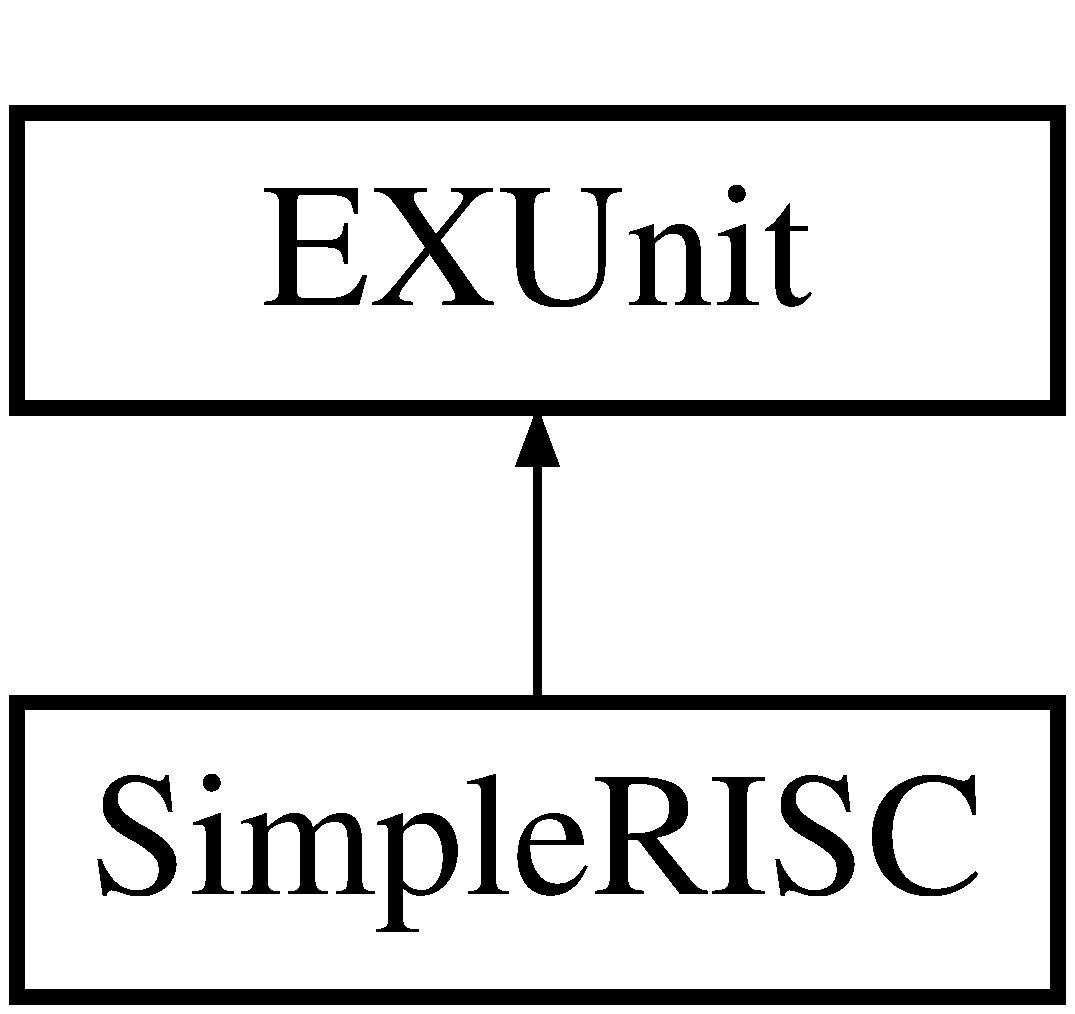
\includegraphics[height=2.000000cm]{class_e_x_unit}
\end{center}
\end{figure}
\subsection*{Entities}
\begin{DoxyCompactItemize}
\item 
\hyperlink{class_e_x_unit_1_1_a_l_u___b_u}{A\-L\-U\-\_\-\-B\-U} architecture
\begin{DoxyCompactList}\small\item\em O\-F\-U is the architectural description of the E\-X Unit. \end{DoxyCompactList}\end{DoxyCompactItemize}
\subsection*{Libraries}
 \begin{DoxyCompactItemize}
\item 
\hypertarget{class_e_x_unit_a0a6af6eef40212dbaf130d57ce711256}{\hyperlink{class_e_x_unit_a0a6af6eef40212dbaf130d57ce711256}{ieee} }\label{class_e_x_unit_a0a6af6eef40212dbaf130d57ce711256}

\end{DoxyCompactItemize}
\subsection*{Use Clauses}
 \begin{DoxyCompactItemize}
\item 
\hypertarget{class_e_x_unit_a43ecb358105806229eb7a3074fc4d577}{\hyperlink{class_e_x_unit_a43ecb358105806229eb7a3074fc4d577}{ieee.\-std\-\_\-logic\-\_\-1164.\-all}   }\label{class_e_x_unit_a43ecb358105806229eb7a3074fc4d577}

\item 
\hypertarget{class_e_x_unit_a631689596594b2068e0ee8dadd0931fe}{\hyperlink{class_e_x_unit_a631689596594b2068e0ee8dadd0931fe}{ieee.\-numeric\-\_\-std.\-all}   }\label{class_e_x_unit_a631689596594b2068e0ee8dadd0931fe}

\end{DoxyCompactItemize}
\subsection*{Ports}
 \begin{DoxyCompactItemize}
\item 
\hypertarget{class_e_x_unit_a38ecec2f0199d6a9ec8272f1afa54b7d}{\hyperlink{class_e_x_unit_a38ecec2f0199d6a9ec8272f1afa54b7d}{op1}  {\bfseries {\bfseries \textcolor{vhdlkeyword}{in}\textcolor{vhdlchar}{ }}} {\bfseries \textcolor{comment}{std\-\_\-logic\-\_\-vector}\textcolor{vhdlchar}{ }\textcolor{vhdlchar}{(}\textcolor{vhdlchar}{ } \textcolor{vhdldigit}{31} \textcolor{vhdlchar}{ }\textcolor{vhdlchar}{ }\textcolor{vhdlchar}{ }\textcolor{vhdlkeyword}{downto}\textcolor{vhdlchar}{ }\textcolor{vhdlchar}{ }\textcolor{vhdlchar}{ } \textcolor{vhdldigit}{0} \textcolor{vhdlchar}{ }\textcolor{vhdlchar}{)}\textcolor{vhdlchar}{ }} }\label{class_e_x_unit_a38ecec2f0199d6a9ec8272f1afa54b7d}

\begin{DoxyCompactList}\small\item\em Operand 1. \end{DoxyCompactList}\item 
\hypertarget{class_e_x_unit_ac695995bed71de6443f520665d1156b1}{\hyperlink{class_e_x_unit_ac695995bed71de6443f520665d1156b1}{op2}  {\bfseries {\bfseries \textcolor{vhdlkeyword}{in}\textcolor{vhdlchar}{ }}} {\bfseries \textcolor{comment}{std\-\_\-logic\-\_\-vector}\textcolor{vhdlchar}{ }\textcolor{vhdlchar}{(}\textcolor{vhdlchar}{ } \textcolor{vhdldigit}{31} \textcolor{vhdlchar}{ }\textcolor{vhdlchar}{ }\textcolor{vhdlchar}{ }\textcolor{vhdlkeyword}{downto}\textcolor{vhdlchar}{ }\textcolor{vhdlchar}{ }\textcolor{vhdlchar}{ } \textcolor{vhdldigit}{0} \textcolor{vhdlchar}{ }\textcolor{vhdlchar}{)}\textcolor{vhdlchar}{ }} }\label{class_e_x_unit_ac695995bed71de6443f520665d1156b1}

\begin{DoxyCompactList}\small\item\em Operand 2. \end{DoxyCompactList}\item 
\hypertarget{class_e_x_unit_a7f6976cd8f8d7c38169b385025f3d04e}{\hyperlink{class_e_x_unit_a7f6976cd8f8d7c38169b385025f3d04e}{immediate}  {\bfseries {\bfseries \textcolor{vhdlkeyword}{in}\textcolor{vhdlchar}{ }}} {\bfseries \textcolor{comment}{std\-\_\-logic\-\_\-vector}\textcolor{vhdlchar}{ }\textcolor{vhdlchar}{(}\textcolor{vhdlchar}{ } \textcolor{vhdldigit}{31} \textcolor{vhdlchar}{ }\textcolor{vhdlchar}{ }\textcolor{vhdlchar}{ }\textcolor{vhdlkeyword}{downto}\textcolor{vhdlchar}{ }\textcolor{vhdlchar}{ }\textcolor{vhdlchar}{ } \textcolor{vhdldigit}{0} \textcolor{vhdlchar}{ }\textcolor{vhdlchar}{)}\textcolor{vhdlchar}{ }} }\label{class_e_x_unit_a7f6976cd8f8d7c38169b385025f3d04e}

\begin{DoxyCompactList}\small\item\em The value of the immediate converted from 27 to 32 bit. \end{DoxyCompactList}\item 
\hypertarget{class_e_x_unit_a8f3e7f694135464cca6480a29fc21731}{\hyperlink{class_e_x_unit_a8f3e7f694135464cca6480a29fc21731}{alu\-S}  {\bfseries {\bfseries \textcolor{vhdlkeyword}{in}\textcolor{vhdlchar}{ }}} {\bfseries \textcolor{comment}{std\-\_\-logic\-\_\-vector}\textcolor{vhdlchar}{ }\textcolor{vhdlchar}{(}\textcolor{vhdlchar}{ } \textcolor{vhdldigit}{2} \textcolor{vhdlchar}{ }\textcolor{vhdlchar}{ }\textcolor{vhdlchar}{ }\textcolor{vhdlkeyword}{downto}\textcolor{vhdlchar}{ }\textcolor{vhdlchar}{ }\textcolor{vhdlchar}{ } \textcolor{vhdldigit}{0} \textcolor{vhdlchar}{ }\textcolor{vhdlchar}{)}\textcolor{vhdlchar}{ }} }\label{class_e_x_unit_a8f3e7f694135464cca6480a29fc21731}

\begin{DoxyCompactList}\small\item\em This vector marks the type of instruction. \end{DoxyCompactList}\item 
\hypertarget{class_e_x_unit_a98da0162bffbb0d8fb2c821dfe215e20}{\hyperlink{class_e_x_unit_a98da0162bffbb0d8fb2c821dfe215e20}{alu\-R}  {\bfseries {\bfseries \textcolor{vhdlkeyword}{out}\textcolor{vhdlchar}{ }}} {\bfseries \textcolor{comment}{std\-\_\-logic\-\_\-vector}\textcolor{vhdlchar}{ }\textcolor{vhdlchar}{(}\textcolor{vhdlchar}{ } \textcolor{vhdldigit}{31} \textcolor{vhdlchar}{ }\textcolor{vhdlchar}{ }\textcolor{vhdlchar}{ }\textcolor{vhdlkeyword}{downto}\textcolor{vhdlchar}{ }\textcolor{vhdlchar}{ }\textcolor{vhdlchar}{ } \textcolor{vhdldigit}{0} \textcolor{vhdlchar}{ }\textcolor{vhdlchar}{)}\textcolor{vhdlchar}{ }} }\label{class_e_x_unit_a98da0162bffbb0d8fb2c821dfe215e20}

\begin{DoxyCompactList}\small\item\em This store the result of the arithmetic operation. \end{DoxyCompactList}\item 
\hypertarget{class_e_x_unit_ad733ef6f5566752744c4f0cf46b531d1}{\hyperlink{class_e_x_unit_ad733ef6f5566752744c4f0cf46b531d1}{is\-Mov}  {\bfseries {\bfseries \textcolor{vhdlkeyword}{in}\textcolor{vhdlchar}{ }}} {\bfseries \textcolor{comment}{boolean}\textcolor{vhdlchar}{ }} }\label{class_e_x_unit_ad733ef6f5566752744c4f0cf46b531d1}

\begin{DoxyCompactList}\small\item\em boolean which states whether the instruction is 'mov' \end{DoxyCompactList}\item 
\hypertarget{class_e_x_unit_acb82c0720fe8e01ce8dfd5412698f724}{\hyperlink{class_e_x_unit_acb82c0720fe8e01ce8dfd5412698f724}{is\-Beq}  {\bfseries {\bfseries \textcolor{vhdlkeyword}{in}\textcolor{vhdlchar}{ }}} {\bfseries \textcolor{comment}{boolean}\textcolor{vhdlchar}{ }} }\label{class_e_x_unit_acb82c0720fe8e01ce8dfd5412698f724}

\begin{DoxyCompactList}\small\item\em boolean which states whether the instruction is 'beq' \end{DoxyCompactList}\item 
\hypertarget{class_e_x_unit_a54b70f333bc66167d7af24c58cd6a779}{\hyperlink{class_e_x_unit_a54b70f333bc66167d7af24c58cd6a779}{is\-Bgt}  {\bfseries {\bfseries \textcolor{vhdlkeyword}{in}\textcolor{vhdlchar}{ }}} {\bfseries \textcolor{comment}{boolean}\textcolor{vhdlchar}{ }} }\label{class_e_x_unit_a54b70f333bc66167d7af24c58cd6a779}

\begin{DoxyCompactList}\small\item\em boolean which states whether the instruction is 'bgt' \end{DoxyCompactList}\item 
\hypertarget{class_e_x_unit_aea0608f12955e6a600f966b0ca7eb6d4}{\hyperlink{class_e_x_unit_aea0608f12955e6a600f966b0ca7eb6d4}{is\-U\-Branch}  {\bfseries {\bfseries \textcolor{vhdlkeyword}{in}\textcolor{vhdlchar}{ }}} {\bfseries \textcolor{comment}{boolean}\textcolor{vhdlchar}{ }} }\label{class_e_x_unit_aea0608f12955e6a600f966b0ca7eb6d4}

\begin{DoxyCompactList}\small\item\em boolean which states whether the instruction is a direct branching statement. \end{DoxyCompactList}\item 
\hypertarget{class_e_x_unit_acc89ba05f91483fee4568ed3da0305b6}{\hyperlink{class_e_x_unit_acc89ba05f91483fee4568ed3da0305b6}{is\-Immediate}  {\bfseries {\bfseries \textcolor{vhdlkeyword}{in}\textcolor{vhdlchar}{ }}} {\bfseries \textcolor{comment}{boolean}\textcolor{vhdlchar}{ }} }\label{class_e_x_unit_acc89ba05f91483fee4568ed3da0305b6}

\begin{DoxyCompactList}\small\item\em boolean which states whether the instruction has an immediate. \end{DoxyCompactList}\item 
\hypertarget{class_e_x_unit_a0add25d9034509d90a2ac075bc1114c1}{\hyperlink{class_e_x_unit_a0add25d9034509d90a2ac075bc1114c1}{is\-Branch\-Taken}  {\bfseries {\bfseries \textcolor{vhdlkeyword}{out}\textcolor{vhdlchar}{ }}} {\bfseries \textcolor{comment}{boolean}\textcolor{vhdlchar}{ }} }\label{class_e_x_unit_a0add25d9034509d90a2ac075bc1114c1}

\begin{DoxyCompactList}\small\item\em boolean whether the branch is taken. \end{DoxyCompactList}\end{DoxyCompactItemize}


\subsection{Detailed Description}
This is the unit that implements the A\-L\-U and branch Unit. 

The documentation for this class was generated from the following file\-:\begin{DoxyCompactItemize}
\item 
\hyperlink{_e_x_unit_8vhdl}{E\-X\-Unit.\-vhdl}\end{DoxyCompactItemize}

\hypertarget{classfile_read}{\section{file\-Read Package Reference}
\label{classfile_read}\index{file\-Read@{file\-Read}}
}


This function converts a char to std\-\_\-logic.  


{\bfseries Package Body $>$$>$ }\hyperlink{class__file_read}{file\-Read}\\*
\subsection*{Functions}
 \begin{DoxyCompactItemize}
\item 
\hypertarget{classfile_read_a130c40cc008de8d3ccb7e18201a712b9}{{\bfseries {\bfseries \textcolor{comment}{std\-\_\-logic}\textcolor{vhdlchar}{ }}} \hyperlink{classfile_read_a130c40cc008de8d3ccb7e18201a712b9}{to\-\_\-std\-\_\-logic\-\_\-from\-\_\-char}{\bfseries  ( }{\bfseries \textcolor{vhdlchar}{data\-: }\textcolor{stringliteral}{in }{\bfseries \textcolor{comment}{character}\textcolor{vhdlchar}{ }}}{\bfseries  )} }\label{classfile_read_a130c40cc008de8d3ccb7e18201a712b9}

\item 
\hypertarget{classfile_read_a2f37cc7e400e439a39996222cc6c4773}{{\bfseries {\bfseries \textcolor{comment}{std\-\_\-logic\-\_\-vector}\textcolor{vhdlchar}{ }}} \hyperlink{classfile_read_a2f37cc7e400e439a39996222cc6c4773}{to\-\_\-std\-\_\-logic\-\_\-vector}{\bfseries  ( }{\bfseries \textcolor{vhdlchar}{data\-: }\textcolor{stringliteral}{in }{\bfseries \textcolor{comment}{string}\textcolor{vhdlchar}{ }}}{\bfseries  )} }\label{classfile_read_a2f37cc7e400e439a39996222cc6c4773}

\begin{DoxyCompactList}\small\item\em This function converts a string to a vector. \end{DoxyCompactList}\end{DoxyCompactItemize}
\subsection*{Libraries}
 \begin{DoxyCompactItemize}
\item 
\hypertarget{classfile_read_ae4f03c286607f3181e16b9aa12d0c6d4}{\hyperlink{classfile_read_ae4f03c286607f3181e16b9aa12d0c6d4}{I\-E\-E\-E} }\label{classfile_read_ae4f03c286607f3181e16b9aa12d0c6d4}

\begin{DoxyCompactList}\small\item\em Whether the instruction is ret,call,b,beq or bgt, this boolean specifies whether the branch is actually taken. \end{DoxyCompactList}\end{DoxyCompactItemize}
\subsection*{Use Clauses}
 \begin{DoxyCompactItemize}
\item 
\hypertarget{classfile_read_a15bb3e73d905716d3f089eda6c1cb112}{\hyperlink{classfile_read_a15bb3e73d905716d3f089eda6c1cb112}{I\-E\-E\-E.\-std\-\_\-logic\-\_\-1164.\-all}   }\label{classfile_read_a15bb3e73d905716d3f089eda6c1cb112}

\end{DoxyCompactItemize}


\subsection{Detailed Description}
This function converts a char to std\-\_\-logic. 

The documentation for this class was generated from the following file\-:\begin{DoxyCompactItemize}
\item 
\hyperlink{file_read_8vhdl}{file\-Read.\-vhdl}\end{DoxyCompactItemize}

\hypertarget{class_i_f_unit}{\section{I\-F\-Unit Entity Reference}
\label{class_i_f_unit}\index{I\-F\-Unit@{I\-F\-Unit}}
}


This is the unit that implements the Instruction fetch Unit.  


Inheritance diagram for I\-F\-Unit\-:\begin{figure}[H]
\begin{center}
\leavevmode
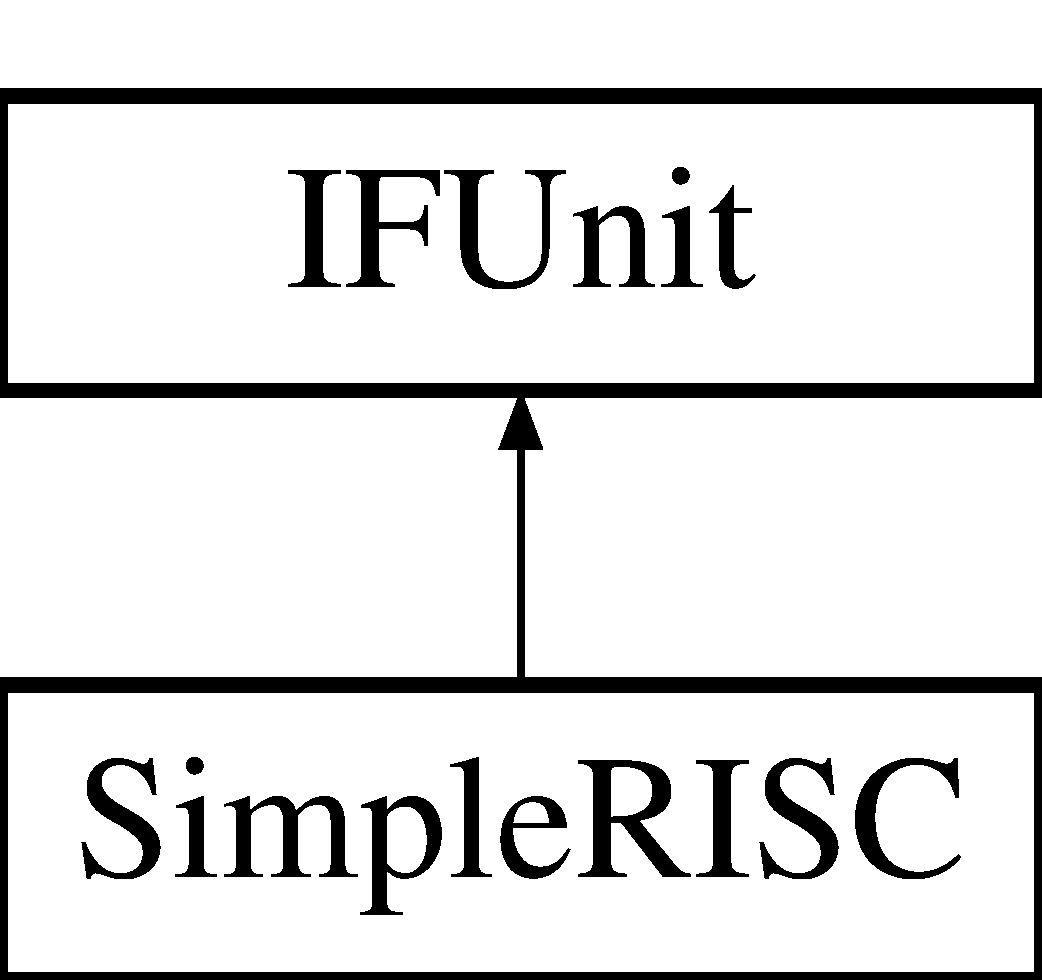
\includegraphics[height=2.000000cm]{class_i_f_unit}
\end{center}
\end{figure}
\subsection*{Entities}
\begin{DoxyCompactItemize}
\item 
\hyperlink{class_i_f_unit_1_1_i_m}{I\-M} architecture
\begin{DoxyCompactList}\small\item\em \hyperlink{class_i_f_unit_1_1_i_m}{I\-M} is the architectural description of the Instruction Fetch Unit. \end{DoxyCompactList}\end{DoxyCompactItemize}
\subsection*{Libraries}
 \begin{DoxyCompactItemize}
\item 
\hypertarget{class_i_f_unit_a0a6af6eef40212dbaf130d57ce711256}{\hyperlink{class_i_f_unit_a0a6af6eef40212dbaf130d57ce711256}{ieee} }\label{class_i_f_unit_a0a6af6eef40212dbaf130d57ce711256}

\item 
\hypertarget{class_i_f_unit_a17a7c5b2be3cba8592e83e385620216b}{\hyperlink{class_i_f_unit_a17a7c5b2be3cba8592e83e385620216b}{std} }\label{class_i_f_unit_a17a7c5b2be3cba8592e83e385620216b}

\end{DoxyCompactItemize}
\subsection*{Use Clauses}
 \begin{DoxyCompactItemize}
\item 
\hypertarget{class_i_f_unit_a43ecb358105806229eb7a3074fc4d577}{\hyperlink{class_i_f_unit_a43ecb358105806229eb7a3074fc4d577}{ieee.\-std\-\_\-logic\-\_\-1164.\-all}   }\label{class_i_f_unit_a43ecb358105806229eb7a3074fc4d577}

\item 
\hypertarget{class_i_f_unit_a7a235ce84abb82b20481281563b754a4}{\hyperlink{class_i_f_unit_a7a235ce84abb82b20481281563b754a4}{std.\-textio.\-all}   }\label{class_i_f_unit_a7a235ce84abb82b20481281563b754a4}

\item 
\hypertarget{class_i_f_unit_a631689596594b2068e0ee8dadd0931fe}{\hyperlink{class_i_f_unit_a631689596594b2068e0ee8dadd0931fe}{ieee.\-numeric\-\_\-std.\-all}   }\label{class_i_f_unit_a631689596594b2068e0ee8dadd0931fe}

\item 
\hypertarget{class_i_f_unit_a04d6b3861e96938512d3dcf21757e289}{\hyperlink{class_i_f_unit_a04d6b3861e96938512d3dcf21757e289}{work.\-file\-Read.\-all}   }\label{class_i_f_unit_a04d6b3861e96938512d3dcf21757e289}

\begin{DoxyCompactList}\small\item\em This import contains the manually defined function to take input from a file. \end{DoxyCompactList}\end{DoxyCompactItemize}
\subsection*{Ports}
 \begin{DoxyCompactItemize}
\item 
\hypertarget{class_i_f_unit_a15b73a10b7d4cf16cdae7729404b05da}{\hyperlink{class_i_f_unit_a15b73a10b7d4cf16cdae7729404b05da}{P\-C}  {\bfseries {\bfseries \textcolor{vhdlkeyword}{in}\textcolor{vhdlchar}{ }}} {\bfseries \textcolor{comment}{std\-\_\-logic\-\_\-vector}\textcolor{vhdlchar}{ }\textcolor{vhdlchar}{(}\textcolor{vhdlchar}{ } \textcolor{vhdldigit}{31} \textcolor{vhdlchar}{ }\textcolor{vhdlchar}{ }\textcolor{vhdlchar}{ }\textcolor{vhdlkeyword}{downto}\textcolor{vhdlchar}{ }\textcolor{vhdlchar}{ }\textcolor{vhdlchar}{ } \textcolor{vhdldigit}{0} \textcolor{vhdlchar}{ }\textcolor{vhdlchar}{)}\textcolor{vhdlchar}{ }} }\label{class_i_f_unit_a15b73a10b7d4cf16cdae7729404b05da}

\begin{DoxyCompactList}\small\item\em The program counter. \end{DoxyCompactList}\item 
\hypertarget{class_i_f_unit_a7282477cc05fbd309237c0768127f042}{\hyperlink{class_i_f_unit_a7282477cc05fbd309237c0768127f042}{instruction}  {\bfseries {\bfseries \textcolor{vhdlkeyword}{out}\textcolor{vhdlchar}{ }}} {\bfseries \textcolor{comment}{std\-\_\-logic\-\_\-vector}\textcolor{vhdlchar}{ }\textcolor{vhdlchar}{(}\textcolor{vhdlchar}{ } \textcolor{vhdldigit}{31} \textcolor{vhdlchar}{ }\textcolor{vhdlchar}{ }\textcolor{vhdlchar}{ }\textcolor{vhdlkeyword}{downto}\textcolor{vhdlchar}{ }\textcolor{vhdlchar}{ }\textcolor{vhdlchar}{ } \textcolor{vhdldigit}{0} \textcolor{vhdlchar}{ }\textcolor{vhdlchar}{)}\textcolor{vhdlchar}{ }} }\label{class_i_f_unit_a7282477cc05fbd309237c0768127f042}

\begin{DoxyCompactList}\small\item\em The 32-\/bit instruction corresponding to the program counter. \end{DoxyCompactList}\end{DoxyCompactItemize}


\subsection{Detailed Description}
This is the unit that implements the Instruction fetch Unit. 

The documentation for this class was generated from the following file\-:\begin{DoxyCompactItemize}
\item 
\hyperlink{_i_f_unit_8vhdl}{I\-F\-Unit.\-vhdl}\end{DoxyCompactItemize}

\hypertarget{class_i_f_unit_1_1_i_m}{\section{I\-M Architecture Reference}
\label{class_i_f_unit_1_1_i_m}\index{I\-M@{I\-M}}
}


\hyperlink{class_i_f_unit_1_1_i_m}{I\-M} is the architectural description of the Instruction Fetch Unit.  


\subsection*{Processes}
 \begin{DoxyCompactItemize}
\item 
\hypertarget{class_i_f_unit_1_1_i_m_ac0b0aa4171471237152f7258fc6cd4ac}{\hyperlink{class_i_f_unit_1_1_i_m_ac0b0aa4171471237152f7258fc6cd4ac}{P\-R\-O\-C\-E\-S\-S\-\_\-1}{\bfseries  ( {\bfseries {\bfseries \hyperlink{class_i_f_unit_a15b73a10b7d4cf16cdae7729404b05da}{P\-C}} \textcolor{vhdlchar}{ }\textcolor{vhdlchar}{ }} )}}\label{class_i_f_unit_1_1_i_m_ac0b0aa4171471237152f7258fc6cd4ac}

\begin{DoxyCompactList}\small\item\em Executes only when the program counter is changed. \end{DoxyCompactList}\end{DoxyCompactItemize}
\subsection*{Types}
 \begin{DoxyCompactItemize}
\item 
\hypertarget{class_i_f_unit_1_1_i_m_a49bac0fe5abc88bc74320eabd2613b1f}{{\bfseries \hyperlink{class_i_f_unit_1_1_i_m_a49bac0fe5abc88bc74320eabd2613b1f}{memorydef}{\bfseries \textcolor{vhdlkeyword}{array}\textcolor{vhdlchar}{ }\textcolor{vhdlchar}{(}\textcolor{vhdlchar}{ }\textcolor{vhdlchar}{ }\textcolor{comment}{integer}\textcolor{vhdlchar}{ }\textcolor{vhdlchar}{range$<$$>$}\textcolor{vhdlchar}{ }\textcolor{vhdlchar}{ }\textcolor{vhdlchar}{ }\textcolor{vhdlchar}{)}\textcolor{vhdlchar}{ }\textcolor{vhdlchar}{ }\textcolor{vhdlkeyword}{of}\textcolor{vhdlchar}{ }\textcolor{comment}{std\-\_\-logic\-\_\-vector}\textcolor{vhdlchar}{ }\textcolor{vhdlchar}{(}\textcolor{vhdlchar}{ } \textcolor{vhdldigit}{31} \textcolor{vhdlchar}{ }\textcolor{vhdlchar}{ }\textcolor{vhdlchar}{ }\textcolor{vhdlkeyword}{downto}\textcolor{vhdlchar}{ }\textcolor{vhdlchar}{ }\textcolor{vhdlchar}{ } \textcolor{vhdldigit}{0} \textcolor{vhdlchar}{ }\textcolor{vhdlchar}{)}\textcolor{vhdlchar}{ }}} }\label{class_i_f_unit_1_1_i_m_a49bac0fe5abc88bc74320eabd2613b1f}

\begin{DoxyCompactList}\small\item\em A custom data type for the memory. \end{DoxyCompactList}\end{DoxyCompactItemize}
\subsection*{Signals}
 \begin{DoxyCompactItemize}
\item 
\hypertarget{class_i_f_unit_1_1_i_m_aff51e4a7013bba9d20b780a6cbb74355}{\hyperlink{class_i_f_unit_1_1_i_m_aff51e4a7013bba9d20b780a6cbb74355}{memory} {\bfseries {\bfseries \hyperlink{class_i_f_unit_1_1_i_m_a49bac0fe5abc88bc74320eabd2613b1f}{memorydef}} \textcolor{vhdlchar}{ }\textcolor{vhdlchar}{(}\textcolor{vhdlchar}{ } \textcolor{vhdldigit}{0} \textcolor{vhdlchar}{ }\textcolor{vhdlchar}{ }\textcolor{vhdlchar}{ }\textcolor{vhdlkeyword}{to}\textcolor{vhdlchar}{ }\textcolor{vhdlchar}{ }\textcolor{vhdlchar}{ } \textcolor{vhdldigit}{499} \textcolor{vhdlchar}{ }\textcolor{vhdlchar}{)}\textcolor{vhdlchar}{ }} }\label{class_i_f_unit_1_1_i_m_aff51e4a7013bba9d20b780a6cbb74355}

\begin{DoxyCompactList}\small\item\em The memory is a 500-\/length array of 32-\/bit vectors,ie, it can handle upto 500 instructions. \end{DoxyCompactList}\item 
\hypertarget{class_i_f_unit_1_1_i_m_ade171b0fc4e5e65e8b838a33506afea3}{\hyperlink{class_i_f_unit_1_1_i_m_ade171b0fc4e5e65e8b838a33506afea3}{max\-Count} {\bfseries \textcolor{comment}{integer}\textcolor{vhdlchar}{ }} }\label{class_i_f_unit_1_1_i_m_ade171b0fc4e5e65e8b838a33506afea3}

\begin{DoxyCompactList}\small\item\em Marks the maximum Program counter. \end{DoxyCompactList}\end{DoxyCompactItemize}


\subsection{Detailed Description}
\hyperlink{class_i_f_unit_1_1_i_m}{I\-M} is the architectural description of the Instruction Fetch Unit. 

The documentation for this class was generated from the following file\-:\begin{DoxyCompactItemize}
\item 
\hyperlink{_i_f_unit_8vhdl}{I\-F\-Unit.\-vhdl}\end{DoxyCompactItemize}

\hypertarget{class_simple_r_i_s_c_1_1main}{\section{main Architecture Reference}
\label{class_simple_r_i_s_c_1_1main}\index{main@{main}}
}
\subsection*{Components}
 \begin{DoxyCompactItemize}
\item 
\hypertarget{class_simple_r_i_s_c_1_1main_a2da5b49da774fb039de79c08078b9c4c}{\hyperlink{class_simple_r_i_s_c_1_1main_a2da5b49da774fb039de79c08078b9c4c}{I\-F\-Unit}  {\bfseries }  }\label{class_simple_r_i_s_c_1_1main_a2da5b49da774fb039de79c08078b9c4c}

\begin{DoxyCompactList}\small\item\em Instruciton Fetch Unit. \end{DoxyCompactList}\item 
\hypertarget{class_simple_r_i_s_c_1_1main_a776fe425523eab02e315d8a4d28e30b7}{\hyperlink{class_simple_r_i_s_c_1_1main_a776fe425523eab02e315d8a4d28e30b7}{C\-Unit}  {\bfseries }  }\label{class_simple_r_i_s_c_1_1main_a776fe425523eab02e315d8a4d28e30b7}

\begin{DoxyCompactList}\small\item\em Constrol Unit. \end{DoxyCompactList}\item 
\hypertarget{class_simple_r_i_s_c_1_1main_ad558d5ce62b24bcc71c1098c3b5252f8}{\hyperlink{class_simple_r_i_s_c_1_1main_ad558d5ce62b24bcc71c1098c3b5252f8}{O\-F\-Unit}  {\bfseries }  }\label{class_simple_r_i_s_c_1_1main_ad558d5ce62b24bcc71c1098c3b5252f8}

\begin{DoxyCompactList}\small\item\em Operand Fetch Unit and Register Write Unit. \end{DoxyCompactList}\item 
\hypertarget{class_simple_r_i_s_c_1_1main_aeeb36d4e2f94902e0f51d5f1e619c3f7}{\hyperlink{class_simple_r_i_s_c_1_1main_aeeb36d4e2f94902e0f51d5f1e619c3f7}{E\-X\-Unit}  {\bfseries }  }\label{class_simple_r_i_s_c_1_1main_aeeb36d4e2f94902e0f51d5f1e619c3f7}

\begin{DoxyCompactList}\small\item\em Execute Unit. \end{DoxyCompactList}\item 
\hypertarget{class_simple_r_i_s_c_1_1main_aad9e7d27bfbe753d62128f7d34d08b15}{\hyperlink{class_simple_r_i_s_c_1_1main_aad9e7d27bfbe753d62128f7d34d08b15}{M\-A\-Unit}  {\bfseries }  }\label{class_simple_r_i_s_c_1_1main_aad9e7d27bfbe753d62128f7d34d08b15}

\begin{DoxyCompactList}\small\item\em Memory access unit. \end{DoxyCompactList}\end{DoxyCompactItemize}
\subsection*{Signals}
 \begin{DoxyCompactItemize}
\item 
\hypertarget{class_simple_r_i_s_c_1_1main_a5857e39b3d56429139fcaba0533d3961}{\hyperlink{class_simple_r_i_s_c_1_1main_a5857e39b3d56429139fcaba0533d3961}{clk} {\bfseries \textcolor{comment}{std\-\_\-logic}\textcolor{vhdlchar}{ }\textcolor{vhdlchar}{ }\textcolor{vhdlchar}{\-:}\textcolor{vhdlchar}{=}\textcolor{vhdlchar}{ }\textcolor{vhdlchar}{'}\textcolor{vhdlchar}{ } \textcolor{vhdldigit}{0} \textcolor{vhdlchar}{ }\textcolor{vhdlchar}{'}\textcolor{vhdlchar}{ }} }\label{class_simple_r_i_s_c_1_1main_a5857e39b3d56429139fcaba0533d3961}

\begin{DoxyCompactList}\small\item\em Clock Signal initialed with 0. \end{DoxyCompactList}\item 
\hypertarget{class_simple_r_i_s_c_1_1main_aa8e9caeeae56e2652cba742bdb6e6e31}{\hyperlink{class_simple_r_i_s_c_1_1main_aa8e9caeeae56e2652cba742bdb6e6e31}{P\-C} {\bfseries \textcolor{comment}{std\-\_\-logic\-\_\-vector}\textcolor{vhdlchar}{ }\textcolor{vhdlchar}{(}\textcolor{vhdlchar}{ } \textcolor{vhdldigit}{31} \textcolor{vhdlchar}{ }\textcolor{vhdlchar}{ }\textcolor{vhdlchar}{ }\textcolor{vhdlkeyword}{downto}\textcolor{vhdlchar}{ }\textcolor{vhdlchar}{ }\textcolor{vhdlchar}{ } \textcolor{vhdldigit}{0} \textcolor{vhdlchar}{ }\textcolor{vhdlchar}{)}\textcolor{vhdlchar}{ }\textcolor{vhdlchar}{ }\textcolor{vhdlchar}{\-:}\textcolor{vhdlchar}{=}\textcolor{vhdlchar}{ }\textcolor{vhdlchar}{X}\textcolor{vhdlchar}{ }\textcolor{keyword}{\char`\"{} F\-F\-F\-F\-F\-F\-F\-C \char`\"{}}\textcolor{vhdlchar}{ }} }\label{class_simple_r_i_s_c_1_1main_aa8e9caeeae56e2652cba742bdb6e6e31}

\begin{DoxyCompactList}\small\item\em Program Counter initialized with -\/4. \end{DoxyCompactList}\item 
\hypertarget{class_simple_r_i_s_c_1_1main_a0a8debbc78ed5d82965045d4eee97461}{\hyperlink{class_simple_r_i_s_c_1_1main_a0a8debbc78ed5d82965045d4eee97461}{instruction} {\bfseries \textcolor{comment}{std\-\_\-logic\-\_\-vector}\textcolor{vhdlchar}{ }\textcolor{vhdlchar}{(}\textcolor{vhdlchar}{ } \textcolor{vhdldigit}{31} \textcolor{vhdlchar}{ }\textcolor{vhdlchar}{ }\textcolor{vhdlchar}{ }\textcolor{vhdlkeyword}{downto}\textcolor{vhdlchar}{ }\textcolor{vhdlchar}{ }\textcolor{vhdlchar}{ } \textcolor{vhdldigit}{0} \textcolor{vhdlchar}{ }\textcolor{vhdlchar}{)}\textcolor{vhdlchar}{ }} }\label{class_simple_r_i_s_c_1_1main_a0a8debbc78ed5d82965045d4eee97461}

\begin{DoxyCompactList}\small\item\em The instruction signal. \end{DoxyCompactList}\item 
\hypertarget{class_simple_r_i_s_c_1_1main_a2a8e68b780117801c3f167ed6ee136a4}{\hyperlink{class_simple_r_i_s_c_1_1main_a2a8e68b780117801c3f167ed6ee136a4}{is\-Mov} {\bfseries \textcolor{comment}{boolean}\textcolor{vhdlchar}{ }\textcolor{vhdlchar}{ }\textcolor{vhdlchar}{\-:}\textcolor{vhdlchar}{=}\textcolor{vhdlchar}{ }\textcolor{vhdlchar}{false}\textcolor{vhdlchar}{ }} }\label{class_simple_r_i_s_c_1_1main_a2a8e68b780117801c3f167ed6ee136a4}

\begin{DoxyCompactList}\small\item\em boolean for mov statement \end{DoxyCompactList}\item 
\hypertarget{class_simple_r_i_s_c_1_1main_a9d22fe433cd653a8faf71c22d73cb47e}{\hyperlink{class_simple_r_i_s_c_1_1main_a9d22fe433cd653a8faf71c22d73cb47e}{is\-St} {\bfseries \textcolor{comment}{boolean}\textcolor{vhdlchar}{ }\textcolor{vhdlchar}{ }\textcolor{vhdlchar}{\-:}\textcolor{vhdlchar}{=}\textcolor{vhdlchar}{ }\textcolor{vhdlchar}{false}\textcolor{vhdlchar}{ }} }\label{class_simple_r_i_s_c_1_1main_a9d22fe433cd653a8faf71c22d73cb47e}

\begin{DoxyCompactList}\small\item\em boolean for store statement \end{DoxyCompactList}\item 
\hypertarget{class_simple_r_i_s_c_1_1main_a153740b434d3545cd8fa0f244ed26498}{\hyperlink{class_simple_r_i_s_c_1_1main_a153740b434d3545cd8fa0f244ed26498}{is\-Ld} {\bfseries \textcolor{comment}{boolean}\textcolor{vhdlchar}{ }\textcolor{vhdlchar}{ }\textcolor{vhdlchar}{\-:}\textcolor{vhdlchar}{=}\textcolor{vhdlchar}{ }\textcolor{vhdlchar}{false}\textcolor{vhdlchar}{ }} }\label{class_simple_r_i_s_c_1_1main_a153740b434d3545cd8fa0f244ed26498}

\begin{DoxyCompactList}\small\item\em boolean for load statement \end{DoxyCompactList}\item 
\hypertarget{class_simple_r_i_s_c_1_1main_a2cb254fbf3f6002a6b69023e4f99c4ef}{\hyperlink{class_simple_r_i_s_c_1_1main_a2cb254fbf3f6002a6b69023e4f99c4ef}{is\-Beq} {\bfseries \textcolor{comment}{boolean}\textcolor{vhdlchar}{ }\textcolor{vhdlchar}{ }\textcolor{vhdlchar}{\-:}\textcolor{vhdlchar}{=}\textcolor{vhdlchar}{ }\textcolor{vhdlchar}{false}\textcolor{vhdlchar}{ }} }\label{class_simple_r_i_s_c_1_1main_a2cb254fbf3f6002a6b69023e4f99c4ef}

\begin{DoxyCompactList}\small\item\em boolean for branch if equal statement \end{DoxyCompactList}\item 
\hypertarget{class_simple_r_i_s_c_1_1main_a2cf6112b9dbca878e9315f777120a60a}{\hyperlink{class_simple_r_i_s_c_1_1main_a2cf6112b9dbca878e9315f777120a60a}{is\-Bgt} {\bfseries \textcolor{comment}{boolean}\textcolor{vhdlchar}{ }\textcolor{vhdlchar}{ }\textcolor{vhdlchar}{\-:}\textcolor{vhdlchar}{=}\textcolor{vhdlchar}{ }\textcolor{vhdlchar}{false}\textcolor{vhdlchar}{ }} }\label{class_simple_r_i_s_c_1_1main_a2cf6112b9dbca878e9315f777120a60a}

\begin{DoxyCompactList}\small\item\em boolean for branch if greater statement \end{DoxyCompactList}\item 
\hypertarget{class_simple_r_i_s_c_1_1main_a74ba3cf06911e5201a3e2f3f32213258}{\hyperlink{class_simple_r_i_s_c_1_1main_a74ba3cf06911e5201a3e2f3f32213258}{is\-Immediate} {\bfseries \textcolor{comment}{boolean}\textcolor{vhdlchar}{ }\textcolor{vhdlchar}{ }\textcolor{vhdlchar}{\-:}\textcolor{vhdlchar}{=}\textcolor{vhdlchar}{ }\textcolor{vhdlchar}{false}\textcolor{vhdlchar}{ }} }\label{class_simple_r_i_s_c_1_1main_a74ba3cf06911e5201a3e2f3f32213258}

\begin{DoxyCompactList}\small\item\em boolean for the statements whre second operand is an immediate \end{DoxyCompactList}\item 
\hypertarget{class_simple_r_i_s_c_1_1main_ad9bc07a81c4a0f0e8290dd663797eaac}{\hyperlink{class_simple_r_i_s_c_1_1main_ad9bc07a81c4a0f0e8290dd663797eaac}{is\-Wb} {\bfseries \textcolor{comment}{boolean}\textcolor{vhdlchar}{ }\textcolor{vhdlchar}{ }\textcolor{vhdlchar}{\-:}\textcolor{vhdlchar}{=}\textcolor{vhdlchar}{ }\textcolor{vhdlchar}{false}\textcolor{vhdlchar}{ }} }\label{class_simple_r_i_s_c_1_1main_ad9bc07a81c4a0f0e8290dd663797eaac}

\begin{DoxyCompactList}\small\item\em boolean for the statements involving writing into register \end{DoxyCompactList}\item 
\hypertarget{class_simple_r_i_s_c_1_1main_a2554956e68f2502184e2b11c6d0bf726}{\hyperlink{class_simple_r_i_s_c_1_1main_a2554956e68f2502184e2b11c6d0bf726}{is\-Ubranch} {\bfseries \textcolor{comment}{boolean}\textcolor{vhdlchar}{ }\textcolor{vhdlchar}{ }\textcolor{vhdlchar}{\-:}\textcolor{vhdlchar}{=}\textcolor{vhdlchar}{ }\textcolor{vhdlchar}{false}\textcolor{vhdlchar}{ }} }\label{class_simple_r_i_s_c_1_1main_a2554956e68f2502184e2b11c6d0bf726}

\begin{DoxyCompactList}\small\item\em boolean for call, ret, b, bgt, beq instructions \end{DoxyCompactList}\item 
\hypertarget{class_simple_r_i_s_c_1_1main_a9febe4603c9484216f7bd07c9ac5465a}{\hyperlink{class_simple_r_i_s_c_1_1main_a9febe4603c9484216f7bd07c9ac5465a}{is\-Branch\-Taken} {\bfseries \textcolor{comment}{boolean}\textcolor{vhdlchar}{ }\textcolor{vhdlchar}{ }\textcolor{vhdlchar}{\-:}\textcolor{vhdlchar}{=}\textcolor{vhdlchar}{ }\textcolor{vhdlchar}{false}\textcolor{vhdlchar}{ }} }\label{class_simple_r_i_s_c_1_1main_a9febe4603c9484216f7bd07c9ac5465a}

\begin{DoxyCompactList}\small\item\em boolean which is true when branch is taken by call, ret, b, bgt, beq instructions \end{DoxyCompactList}\item 
\hypertarget{class_simple_r_i_s_c_1_1main_a4326436a10c51413d01ebb2c8ab4d9a6}{\hyperlink{class_simple_r_i_s_c_1_1main_a4326436a10c51413d01ebb2c8ab4d9a6}{is\-Ret} {\bfseries \textcolor{comment}{boolean}\textcolor{vhdlchar}{ }\textcolor{vhdlchar}{ }\textcolor{vhdlchar}{\-:}\textcolor{vhdlchar}{=}\textcolor{vhdlchar}{ }\textcolor{vhdlchar}{false}\textcolor{vhdlchar}{ }} }\label{class_simple_r_i_s_c_1_1main_a4326436a10c51413d01ebb2c8ab4d9a6}

\begin{DoxyCompactList}\small\item\em boolean for ret instruction \end{DoxyCompactList}\item 
\hypertarget{class_simple_r_i_s_c_1_1main_a374d3926d6376e22fc6ef74d586f36ea}{\hyperlink{class_simple_r_i_s_c_1_1main_a374d3926d6376e22fc6ef74d586f36ea}{is\-Call} {\bfseries \textcolor{comment}{boolean}\textcolor{vhdlchar}{ }\textcolor{vhdlchar}{ }\textcolor{vhdlchar}{\-:}\textcolor{vhdlchar}{=}\textcolor{vhdlchar}{ }\textcolor{vhdlchar}{false}\textcolor{vhdlchar}{ }} }\label{class_simple_r_i_s_c_1_1main_a374d3926d6376e22fc6ef74d586f36ea}

\begin{DoxyCompactList}\small\item\em boolean for call instruction \end{DoxyCompactList}\item 
\hypertarget{class_simple_r_i_s_c_1_1main_a6ec50893678c7daa0e7fe1c555e11a08}{\hyperlink{class_simple_r_i_s_c_1_1main_a6ec50893678c7daa0e7fe1c555e11a08}{alu\-S} {\bfseries \textcolor{comment}{std\-\_\-logic\-\_\-vector}\textcolor{vhdlchar}{ }\textcolor{vhdlchar}{(}\textcolor{vhdlchar}{ } \textcolor{vhdldigit}{2} \textcolor{vhdlchar}{ }\textcolor{vhdlchar}{ }\textcolor{vhdlchar}{ }\textcolor{vhdlkeyword}{downto}\textcolor{vhdlchar}{ }\textcolor{vhdlchar}{ }\textcolor{vhdlchar}{ } \textcolor{vhdldigit}{0} \textcolor{vhdlchar}{ }\textcolor{vhdlchar}{)}\textcolor{vhdlchar}{ }} }\label{class_simple_r_i_s_c_1_1main_a6ec50893678c7daa0e7fe1c555e11a08}

\begin{DoxyCompactList}\small\item\em A\-L\-U Signals generated by the Control Unit for A\-L\-U to perform adequate operation. \end{DoxyCompactList}\item 
\hypertarget{class_simple_r_i_s_c_1_1main_a2c7c7c5cf1af62fc1be6fb1c55c9b864}{\hyperlink{class_simple_r_i_s_c_1_1main_a2c7c7c5cf1af62fc1be6fb1c55c9b864}{alu\-R} {\bfseries \textcolor{comment}{std\-\_\-logic\-\_\-vector}\textcolor{vhdlchar}{ }\textcolor{vhdlchar}{(}\textcolor{vhdlchar}{ } \textcolor{vhdldigit}{31} \textcolor{vhdlchar}{ }\textcolor{vhdlchar}{ }\textcolor{vhdlchar}{ }\textcolor{vhdlkeyword}{downto}\textcolor{vhdlchar}{ }\textcolor{vhdlchar}{ }\textcolor{vhdlchar}{ } \textcolor{vhdldigit}{0} \textcolor{vhdlchar}{ }\textcolor{vhdlchar}{)}\textcolor{vhdlchar}{ }\textcolor{vhdlchar}{ }\textcolor{vhdlchar}{\-:}\textcolor{vhdlchar}{=}\textcolor{vhdlchar}{ }\textcolor{vhdlchar}{X}\textcolor{vhdlchar}{ }\textcolor{keyword}{\char`\"{} 00000000 \char`\"{}}\textcolor{vhdlchar}{ }} }\label{class_simple_r_i_s_c_1_1main_a2c7c7c5cf1af62fc1be6fb1c55c9b864}

\begin{DoxyCompactList}\small\item\em Result of the operation by A\-L\-U. \end{DoxyCompactList}\item 
\hypertarget{class_simple_r_i_s_c_1_1main_ab5d29364b579ec10e34fc0befc7fb13b}{\hyperlink{class_simple_r_i_s_c_1_1main_ab5d29364b579ec10e34fc0befc7fb13b}{ld\-R} {\bfseries \textcolor{comment}{std\-\_\-logic\-\_\-vector}\textcolor{vhdlchar}{ }\textcolor{vhdlchar}{(}\textcolor{vhdlchar}{ } \textcolor{vhdldigit}{31} \textcolor{vhdlchar}{ }\textcolor{vhdlchar}{ }\textcolor{vhdlchar}{ }\textcolor{vhdlkeyword}{downto}\textcolor{vhdlchar}{ }\textcolor{vhdlchar}{ }\textcolor{vhdlchar}{ } \textcolor{vhdldigit}{0} \textcolor{vhdlchar}{ }\textcolor{vhdlchar}{)}\textcolor{vhdlchar}{ }\textcolor{vhdlchar}{ }\textcolor{vhdlchar}{\-:}\textcolor{vhdlchar}{=}\textcolor{vhdlchar}{ }\textcolor{vhdlchar}{X}\textcolor{vhdlchar}{ }\textcolor{keyword}{\char`\"{} 00000000 \char`\"{}}\textcolor{vhdlchar}{ }} }\label{class_simple_r_i_s_c_1_1main_ab5d29364b579ec10e34fc0befc7fb13b}

\begin{DoxyCompactList}\small\item\em value read from register file \end{DoxyCompactList}\item 
\hypertarget{class_simple_r_i_s_c_1_1main_a5487b623285f43fb095d9215681d2b34}{\hyperlink{class_simple_r_i_s_c_1_1main_a5487b623285f43fb095d9215681d2b34}{immediate} {\bfseries \textcolor{comment}{std\-\_\-logic\-\_\-vector}\textcolor{vhdlchar}{ }\textcolor{vhdlchar}{(}\textcolor{vhdlchar}{ } \textcolor{vhdldigit}{31} \textcolor{vhdlchar}{ }\textcolor{vhdlchar}{ }\textcolor{vhdlchar}{ }\textcolor{vhdlkeyword}{downto}\textcolor{vhdlchar}{ }\textcolor{vhdlchar}{ }\textcolor{vhdlchar}{ } \textcolor{vhdldigit}{0} \textcolor{vhdlchar}{ }\textcolor{vhdlchar}{)}\textcolor{vhdlchar}{ }\textcolor{vhdlchar}{ }\textcolor{vhdlchar}{\-:}\textcolor{vhdlchar}{=}\textcolor{vhdlchar}{ }\textcolor{vhdlchar}{X}\textcolor{vhdlchar}{ }\textcolor{keyword}{\char`\"{} 00000000 \char`\"{}}\textcolor{vhdlchar}{ }} }\label{class_simple_r_i_s_c_1_1main_a5487b623285f43fb095d9215681d2b34}

\begin{DoxyCompactList}\small\item\em immediate computer after applying modifiers and bit extension \end{DoxyCompactList}\item 
\hypertarget{class_simple_r_i_s_c_1_1main_ad010267538d4e382f6edbf4942a81e9a}{\hyperlink{class_simple_r_i_s_c_1_1main_ad010267538d4e382f6edbf4942a81e9a}{branch\-Target} {\bfseries \textcolor{comment}{std\-\_\-logic\-\_\-vector}\textcolor{vhdlchar}{ }\textcolor{vhdlchar}{(}\textcolor{vhdlchar}{ } \textcolor{vhdldigit}{31} \textcolor{vhdlchar}{ }\textcolor{vhdlchar}{ }\textcolor{vhdlchar}{ }\textcolor{vhdlkeyword}{downto}\textcolor{vhdlchar}{ }\textcolor{vhdlchar}{ }\textcolor{vhdlchar}{ } \textcolor{vhdldigit}{0} \textcolor{vhdlchar}{ }\textcolor{vhdlchar}{)}\textcolor{vhdlchar}{ }\textcolor{vhdlchar}{ }\textcolor{vhdlchar}{\-:}\textcolor{vhdlchar}{=}\textcolor{vhdlchar}{ }\textcolor{vhdlchar}{X}\textcolor{vhdlchar}{ }\textcolor{keyword}{\char`\"{} 00000000 \char`\"{}}\textcolor{vhdlchar}{ }} }\label{class_simple_r_i_s_c_1_1main_ad010267538d4e382f6edbf4942a81e9a}

\begin{DoxyCompactList}\small\item\em brach target computed after adding offset to the program counter \end{DoxyCompactList}\item 
\hypertarget{class_simple_r_i_s_c_1_1main_a168a397ec8f905d38285e1f9832ab64f}{\hyperlink{class_simple_r_i_s_c_1_1main_a168a397ec8f905d38285e1f9832ab64f}{op1} {\bfseries \textcolor{comment}{std\-\_\-logic\-\_\-vector}\textcolor{vhdlchar}{ }\textcolor{vhdlchar}{(}\textcolor{vhdlchar}{ } \textcolor{vhdldigit}{31} \textcolor{vhdlchar}{ }\textcolor{vhdlchar}{ }\textcolor{vhdlchar}{ }\textcolor{vhdlkeyword}{downto}\textcolor{vhdlchar}{ }\textcolor{vhdlchar}{ }\textcolor{vhdlchar}{ } \textcolor{vhdldigit}{0} \textcolor{vhdlchar}{ }\textcolor{vhdlchar}{)}\textcolor{vhdlchar}{ }\textcolor{vhdlchar}{ }\textcolor{vhdlchar}{\-:}\textcolor{vhdlchar}{=}\textcolor{vhdlchar}{ }\textcolor{vhdlchar}{X}\textcolor{vhdlchar}{ }\textcolor{keyword}{\char`\"{} 00000000 \char`\"{}}\textcolor{vhdlchar}{ }} }\label{class_simple_r_i_s_c_1_1main_a168a397ec8f905d38285e1f9832ab64f}

\begin{DoxyCompactList}\small\item\em Fisrt Operand. \end{DoxyCompactList}\item 
\hypertarget{class_simple_r_i_s_c_1_1main_a4596ed60c0f2bc645ff64fa8c8ae66ac}{\hyperlink{class_simple_r_i_s_c_1_1main_a4596ed60c0f2bc645ff64fa8c8ae66ac}{op2} {\bfseries \textcolor{comment}{std\-\_\-logic\-\_\-vector}\textcolor{vhdlchar}{ }\textcolor{vhdlchar}{(}\textcolor{vhdlchar}{ } \textcolor{vhdldigit}{31} \textcolor{vhdlchar}{ }\textcolor{vhdlchar}{ }\textcolor{vhdlchar}{ }\textcolor{vhdlkeyword}{downto}\textcolor{vhdlchar}{ }\textcolor{vhdlchar}{ }\textcolor{vhdlchar}{ } \textcolor{vhdldigit}{0} \textcolor{vhdlchar}{ }\textcolor{vhdlchar}{)}\textcolor{vhdlchar}{ }\textcolor{vhdlchar}{ }\textcolor{vhdlchar}{\-:}\textcolor{vhdlchar}{=}\textcolor{vhdlchar}{ }\textcolor{vhdlchar}{X}\textcolor{vhdlchar}{ }\textcolor{keyword}{\char`\"{} 00000000 \char`\"{}}\textcolor{vhdlchar}{ }} }\label{class_simple_r_i_s_c_1_1main_a4596ed60c0f2bc645ff64fa8c8ae66ac}

\begin{DoxyCompactList}\small\item\em Second Operand. \end{DoxyCompactList}\end{DoxyCompactItemize}
\subsection*{Instantiations}
 \begin{DoxyCompactItemize}
\item 
\hypertarget{class_simple_r_i_s_c_1_1main_a6915378535caef0a1f9d2cf97dc464b7}{\hyperlink{class_simple_r_i_s_c_1_1main_a6915378535caef0a1f9d2cf97dc464b7}{iif}  {\bfseries I\-F\-Unit}   }\label{class_simple_r_i_s_c_1_1main_a6915378535caef0a1f9d2cf97dc464b7}

\begin{DoxyCompactList}\small\item\em maps the signals to the ports of \hyperlink{class_i_f_unit}{I\-F\-Unit} \end{DoxyCompactList}\item 
\hypertarget{class_simple_r_i_s_c_1_1main_ae66107dcb400a2c22d4d1316a2de3289}{\hyperlink{class_simple_r_i_s_c_1_1main_ae66107dcb400a2c22d4d1316a2de3289}{icu}  {\bfseries C\-Unit}   }\label{class_simple_r_i_s_c_1_1main_ae66107dcb400a2c22d4d1316a2de3289}

\begin{DoxyCompactList}\small\item\em maps the signals to the ports of \hyperlink{class_c_unit}{C\-Unit} \end{DoxyCompactList}\item 
\hypertarget{class_simple_r_i_s_c_1_1main_af2805cb31aa7733a71e2d9b7e59bb510}{\hyperlink{class_simple_r_i_s_c_1_1main_af2805cb31aa7733a71e2d9b7e59bb510}{iof}  {\bfseries O\-F\-Unit}   }\label{class_simple_r_i_s_c_1_1main_af2805cb31aa7733a71e2d9b7e59bb510}

\begin{DoxyCompactList}\small\item\em maps the signals to the ports of \hyperlink{class_o_f_unit}{O\-F\-Unit} \end{DoxyCompactList}\item 
\hypertarget{class_simple_r_i_s_c_1_1main_a03911597d8f737c88f243be080110a60}{\hyperlink{class_simple_r_i_s_c_1_1main_a03911597d8f737c88f243be080110a60}{iex}  {\bfseries E\-X\-Unit}   }\label{class_simple_r_i_s_c_1_1main_a03911597d8f737c88f243be080110a60}

\begin{DoxyCompactList}\small\item\em maps the signals to the ports of \hyperlink{class_e_x_unit}{E\-X\-Unit} \end{DoxyCompactList}\item 
\hypertarget{class_simple_r_i_s_c_1_1main_a35c82dc98430213354cf872354a1ca6b}{\hyperlink{class_simple_r_i_s_c_1_1main_a35c82dc98430213354cf872354a1ca6b}{ima}  {\bfseries M\-A\-Unit}   }\label{class_simple_r_i_s_c_1_1main_a35c82dc98430213354cf872354a1ca6b}

\begin{DoxyCompactList}\small\item\em maps the signals to the ports of \hyperlink{class_m_a_unit}{M\-A\-Unit} \end{DoxyCompactList}\end{DoxyCompactItemize}


\subsection{Detailed Description}
This is main assembly of all the components of the prcessor. This is also responsible for generation of clock signal which is sent to all the other components. Further, program counter is also updated in this architecure description only. 

The documentation for this class was generated from the following file\-:\begin{DoxyCompactItemize}
\item 
\hyperlink{_simple_r_i_s_c_8vhdl}{Simple\-R\-I\-S\-C.\-vhdl}\end{DoxyCompactItemize}

\hypertarget{class_m_a_unit}{\section{M\-A\-Unit Entity Reference}
\label{class_m_a_unit}\index{M\-A\-Unit@{M\-A\-Unit}}
}


This is the unit that implements a R\-A\-M.  


Inheritance diagram for M\-A\-Unit\-:\begin{figure}[H]
\begin{center}
\leavevmode
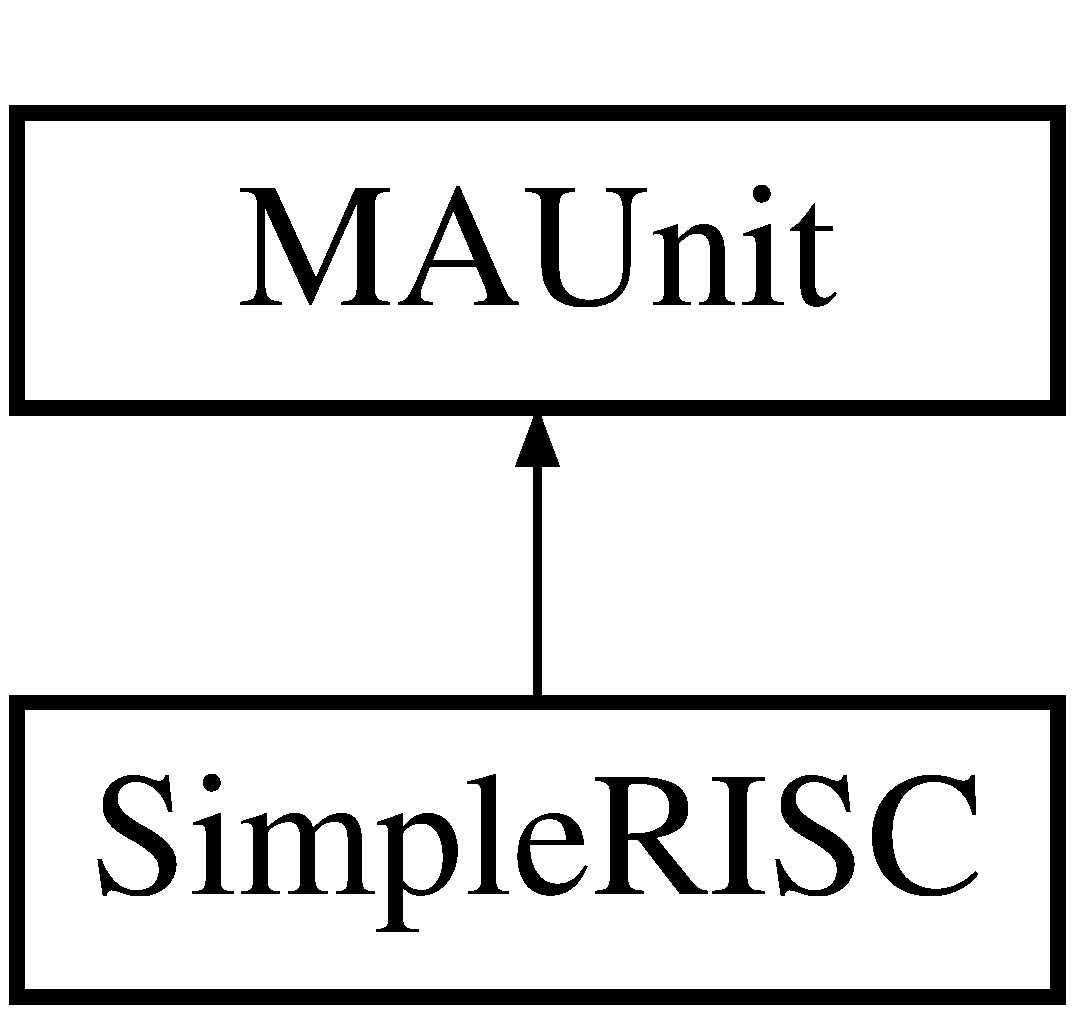
\includegraphics[height=2.000000cm]{class_m_a_unit}
\end{center}
\end{figure}
\subsection*{Entities}
\begin{DoxyCompactItemize}
\item 
\hyperlink{class_m_a_unit_1_1_d_m}{D\-M} architecture
\begin{DoxyCompactList}\small\item\em \hyperlink{class_m_a_unit_1_1_d_m}{D\-M} is the architecture of the Memory Unit. \end{DoxyCompactList}\end{DoxyCompactItemize}
\subsection*{Libraries}
 \begin{DoxyCompactItemize}
\item 
\hypertarget{class_m_a_unit_a0a6af6eef40212dbaf130d57ce711256}{\hyperlink{class_m_a_unit_a0a6af6eef40212dbaf130d57ce711256}{ieee} }\label{class_m_a_unit_a0a6af6eef40212dbaf130d57ce711256}

\end{DoxyCompactItemize}
\subsection*{Use Clauses}
 \begin{DoxyCompactItemize}
\item 
\hypertarget{class_m_a_unit_a43ecb358105806229eb7a3074fc4d577}{\hyperlink{class_m_a_unit_a43ecb358105806229eb7a3074fc4d577}{ieee.\-std\-\_\-logic\-\_\-1164.\-all}   }\label{class_m_a_unit_a43ecb358105806229eb7a3074fc4d577}

\item 
\hypertarget{class_m_a_unit_a631689596594b2068e0ee8dadd0931fe}{\hyperlink{class_m_a_unit_a631689596594b2068e0ee8dadd0931fe}{ieee.\-numeric\-\_\-std.\-all}   }\label{class_m_a_unit_a631689596594b2068e0ee8dadd0931fe}

\end{DoxyCompactItemize}
\subsection*{Ports}
 \begin{DoxyCompactItemize}
\item 
\hypertarget{class_m_a_unit_a94f6b72ef22091aa46807c9d89632a9b}{\hyperlink{class_m_a_unit_a94f6b72ef22091aa46807c9d89632a9b}{clk}  {\bfseries {\bfseries \textcolor{vhdlkeyword}{in}\textcolor{vhdlchar}{ }}} {\bfseries \textcolor{comment}{std\-\_\-logic}\textcolor{vhdlchar}{ }} }\label{class_m_a_unit_a94f6b72ef22091aa46807c9d89632a9b}

\begin{DoxyCompactList}\small\item\em clk is the C\-L\-O\-C\-K coming the the unit \end{DoxyCompactList}\item 
\hypertarget{class_m_a_unit_ac695995bed71de6443f520665d1156b1}{\hyperlink{class_m_a_unit_ac695995bed71de6443f520665d1156b1}{op2}  {\bfseries {\bfseries \textcolor{vhdlkeyword}{in}\textcolor{vhdlchar}{ }}} {\bfseries \textcolor{comment}{std\-\_\-logic\-\_\-vector}\textcolor{vhdlchar}{ }\textcolor{vhdlchar}{(}\textcolor{vhdlchar}{ } \textcolor{vhdldigit}{31} \textcolor{vhdlchar}{ }\textcolor{vhdlchar}{ }\textcolor{vhdlchar}{ }\textcolor{vhdlkeyword}{downto}\textcolor{vhdlchar}{ }\textcolor{vhdlchar}{ }\textcolor{vhdlchar}{ } \textcolor{vhdldigit}{0} \textcolor{vhdlchar}{ }\textcolor{vhdlchar}{)}\textcolor{vhdlchar}{ }} }\label{class_m_a_unit_ac695995bed71de6443f520665d1156b1}

\begin{DoxyCompactList}\small\item\em The value to stored in case of a store instruction. \end{DoxyCompactList}\item 
\hypertarget{class_m_a_unit_a15f3af98c390c64fec95e54717345647}{\hyperlink{class_m_a_unit_a15f3af98c390c64fec95e54717345647}{alu\-R}  {\bfseries {\bfseries \textcolor{vhdlkeyword}{in}\textcolor{vhdlchar}{ }}} {\bfseries \textcolor{comment}{std\-\_\-logic\-\_\-vector}\textcolor{vhdlchar}{ }\textcolor{vhdlchar}{(}\textcolor{vhdlchar}{ } \textcolor{vhdldigit}{31} \textcolor{vhdlchar}{ }\textcolor{vhdlchar}{ }\textcolor{vhdlchar}{ }\textcolor{vhdlkeyword}{downto}\textcolor{vhdlchar}{ }\textcolor{vhdlchar}{ }\textcolor{vhdlchar}{ } \textcolor{vhdldigit}{0} \textcolor{vhdlchar}{ }\textcolor{vhdlchar}{)}\textcolor{vhdlchar}{ }} }\label{class_m_a_unit_a15f3af98c390c64fec95e54717345647}

\begin{DoxyCompactList}\small\item\em alu\-R stores the address of the memory location to be accessed \end{DoxyCompactList}\item 
\hypertarget{class_m_a_unit_ada232e9bb13e48ba67c49897a8f2a98c}{\hyperlink{class_m_a_unit_ada232e9bb13e48ba67c49897a8f2a98c}{is\-St}  {\bfseries {\bfseries \textcolor{vhdlkeyword}{in}\textcolor{vhdlchar}{ }}} {\bfseries \textcolor{comment}{boolean}\textcolor{vhdlchar}{ }} }\label{class_m_a_unit_ada232e9bb13e48ba67c49897a8f2a98c}

\begin{DoxyCompactList}\small\item\em a boolean signal generated by Control Unit to determine if this is a store instruction \end{DoxyCompactList}\item 
\hypertarget{class_m_a_unit_a4f328a19e16850a109722d3bf847ea76}{\hyperlink{class_m_a_unit_a4f328a19e16850a109722d3bf847ea76}{is\-Ld}  {\bfseries {\bfseries \textcolor{vhdlkeyword}{in}\textcolor{vhdlchar}{ }}} {\bfseries \textcolor{comment}{boolean}\textcolor{vhdlchar}{ }} }\label{class_m_a_unit_a4f328a19e16850a109722d3bf847ea76}

\begin{DoxyCompactList}\small\item\em a boolean signal generated by Control Unit to determine if this is a load instruction \end{DoxyCompactList}\item 
\hypertarget{class_m_a_unit_ac062d1d1a95ee963e9211cbe1c9f7574}{\hyperlink{class_m_a_unit_ac062d1d1a95ee963e9211cbe1c9f7574}{ld\-Result}  {\bfseries {\bfseries \textcolor{vhdlkeyword}{out}\textcolor{vhdlchar}{ }}} {\bfseries \textcolor{comment}{std\-\_\-logic\-\_\-vector}\textcolor{vhdlchar}{ }\textcolor{vhdlchar}{(}\textcolor{vhdlchar}{ } \textcolor{vhdldigit}{31} \textcolor{vhdlchar}{ }\textcolor{vhdlchar}{ }\textcolor{vhdlchar}{ }\textcolor{vhdlkeyword}{downto}\textcolor{vhdlchar}{ }\textcolor{vhdlchar}{ }\textcolor{vhdlchar}{ } \textcolor{vhdldigit}{0} \textcolor{vhdlchar}{ }\textcolor{vhdlchar}{)}\textcolor{vhdlchar}{ }} }\label{class_m_a_unit_ac062d1d1a95ee963e9211cbe1c9f7574}

\begin{DoxyCompactList}\small\item\em output signal which contains the value stored in the memory location accessed in case of a load instruction \end{DoxyCompactList}\end{DoxyCompactItemize}


\subsection{Detailed Description}
This is the unit that implements a R\-A\-M. 

The documentation for this class was generated from the following file\-:\begin{DoxyCompactItemize}
\item 
\hyperlink{_m_a_unit_8vhdl}{M\-A\-Unit.\-vhdl}\end{DoxyCompactItemize}

\hypertarget{class_o_f_unit_1_1_o_f_u}{\section{O\-F\-U Architecture Reference}
\label{class_o_f_unit_1_1_o_f_u}\index{O\-F\-U@{O\-F\-U}}
}


\hyperlink{class_o_f_unit_1_1_o_f_u}{O\-F\-U} is the architectural description of the operand fetch unit and register file.  


\subsection*{Processes}
 \begin{DoxyCompactItemize}
\item 
\hyperlink{class_o_f_unit_1_1_o_f_u_ad6cab3590f19d09760591444870d2e29}{P\-R\-O\-C\-E\-S\-S\-\_\-3}{\bfseries  (  )}
\end{DoxyCompactItemize}
\subsection*{Types}
 \begin{DoxyCompactItemize}
\item 
\hypertarget{class_o_f_unit_1_1_o_f_u_a7214ee86d8486f4a264c9251cb623069}{{\bfseries \hyperlink{class_o_f_unit_1_1_o_f_u_a7214ee86d8486f4a264c9251cb623069}{regvec}{\bfseries \textcolor{vhdlkeyword}{array}\textcolor{vhdlchar}{ }\textcolor{vhdlchar}{(}\textcolor{vhdlchar}{ } \textcolor{vhdldigit}{15} \textcolor{vhdlchar}{ }\textcolor{vhdlchar}{ }\textcolor{vhdlchar}{ }\textcolor{vhdlkeyword}{downto}\textcolor{vhdlchar}{ }\textcolor{vhdlchar}{ }\textcolor{vhdlchar}{ } \textcolor{vhdldigit}{0} \textcolor{vhdlchar}{ }\textcolor{vhdlchar}{)}\textcolor{vhdlchar}{ }\textcolor{vhdlchar}{ }\textcolor{vhdlkeyword}{of}\textcolor{vhdlchar}{ }\textcolor{comment}{std\-\_\-logic\-\_\-vector}\textcolor{vhdlchar}{ }\textcolor{vhdlchar}{(}\textcolor{vhdlchar}{ } \textcolor{vhdldigit}{31} \textcolor{vhdlchar}{ }\textcolor{vhdlchar}{ }\textcolor{vhdlchar}{ }\textcolor{vhdlkeyword}{downto}\textcolor{vhdlchar}{ }\textcolor{vhdlchar}{ }\textcolor{vhdlchar}{ } \textcolor{vhdldigit}{0} \textcolor{vhdlchar}{ }\textcolor{vhdlchar}{)}\textcolor{vhdlchar}{ }}} }\label{class_o_f_unit_1_1_o_f_u_a7214ee86d8486f4a264c9251cb623069}

\begin{DoxyCompactList}\small\item\em A custom data type which is a 16 x 32 array or vector of bits. \end{DoxyCompactList}\end{DoxyCompactItemize}
\subsection*{Signals}
 \begin{DoxyCompactItemize}
\item 
\hypertarget{class_o_f_unit_1_1_o_f_u_aad72c6f18f2ed17dab71807f9fcf8778}{\hyperlink{class_o_f_unit_1_1_o_f_u_aad72c6f18f2ed17dab71807f9fcf8778}{reg} {\bfseries {\bfseries \hyperlink{class_o_f_unit_1_1_o_f_u_a7214ee86d8486f4a264c9251cb623069}{regvec}} \textcolor{vhdlchar}{ }} }\label{class_o_f_unit_1_1_o_f_u_aad72c6f18f2ed17dab71807f9fcf8778}

\begin{DoxyCompactList}\small\item\em reg is the register file of data type regvec that is it has 16 32-\/bit vector fields \end{DoxyCompactList}\item 
\hypertarget{class_o_f_unit_1_1_o_f_u_a981d141369765d0e214128c4f3d8ecbb}{\hyperlink{class_o_f_unit_1_1_o_f_u_a981d141369765d0e214128c4f3d8ecbb}{temp} {\bfseries \textcolor{comment}{std\-\_\-logic\-\_\-vector}\textcolor{vhdlchar}{ }\textcolor{vhdlchar}{(}\textcolor{vhdlchar}{ } \textcolor{vhdldigit}{31} \textcolor{vhdlchar}{ }\textcolor{vhdlchar}{ }\textcolor{vhdlchar}{ }\textcolor{vhdlkeyword}{downto}\textcolor{vhdlchar}{ }\textcolor{vhdlchar}{ }\textcolor{vhdlchar}{ } \textcolor{vhdldigit}{0} \textcolor{vhdlchar}{ }\textcolor{vhdlchar}{)}\textcolor{vhdlchar}{ }} }\label{class_o_f_unit_1_1_o_f_u_a981d141369765d0e214128c4f3d8ecbb}

\begin{DoxyCompactList}\small\item\em temp is the signal which is used for signed extension of offset, offset is Instruction(26 downto 0) \end{DoxyCompactList}\end{DoxyCompactItemize}


\subsection{Detailed Description}
\hyperlink{class_o_f_unit_1_1_o_f_u}{O\-F\-U} is the architectural description of the operand fetch unit and register file. 

\subsection{Member Function Documentation}
\hypertarget{class_o_f_unit_1_1_o_f_u_ad6cab3590f19d09760591444870d2e29}{\index{O\-F\-Unit\-::\-O\-F\-U@{O\-F\-Unit\-::\-O\-F\-U}!P\-R\-O\-C\-E\-S\-S\-\_\-3@{P\-R\-O\-C\-E\-S\-S\-\_\-3}}
\index{P\-R\-O\-C\-E\-S\-S\-\_\-3@{P\-R\-O\-C\-E\-S\-S\-\_\-3}!OFUnit::OFU@{O\-F\-Unit\-::\-O\-F\-U}}
\subsubsection[{P\-R\-O\-C\-E\-S\-S\-\_\-3}]{\setlength{\rightskip}{0pt plus 5cm} {\bfseries \textcolor{vhdlchar}{ }} P\-R\-O\-C\-E\-S\-S\-\_\-3 ( ) \hspace{0.3cm}{\ttfamily [Process]}}}\label{class_o_f_unit_1_1_o_f_u_ad6cab3590f19d09760591444870d2e29}
First of all immediate is computed after sign extesnion, if 17th bit of the instruction is 1 then sign extension is not done and if the 18th bit is 1 then the 16-\/bit immediate is shifted left by 16 bits to get the modified immidiate. The branch targeet is computer as $<$ program counter + 4 $\ast$ offset $>$ offset is stored as Instruction(15 downto 0). Frst operand is computer as reg(rs1) where rs1 is stored in Instruction(21 downto 18). Second operand is either reg(rs2) where rs1 is stored in Instruction(17 downto 14) or it is reg(rd) in case of a store instruction where rd is stored as Instruction(25 downto 22). 

The documentation for this class was generated from the following file\-:\begin{DoxyCompactItemize}
\item 
\hyperlink{_o_f_unit_8vhdl}{O\-F\-Unit.\-vhdl}\end{DoxyCompactItemize}

\hypertarget{class_o_f_unit}{\section{O\-F\-Unit Entity Reference}
\label{class_o_f_unit}\index{O\-F\-Unit@{O\-F\-Unit}}
}


This the Operand Fetch Unit which also contains the register file implementation.  


Inheritance diagram for O\-F\-Unit\-:\begin{figure}[H]
\begin{center}
\leavevmode
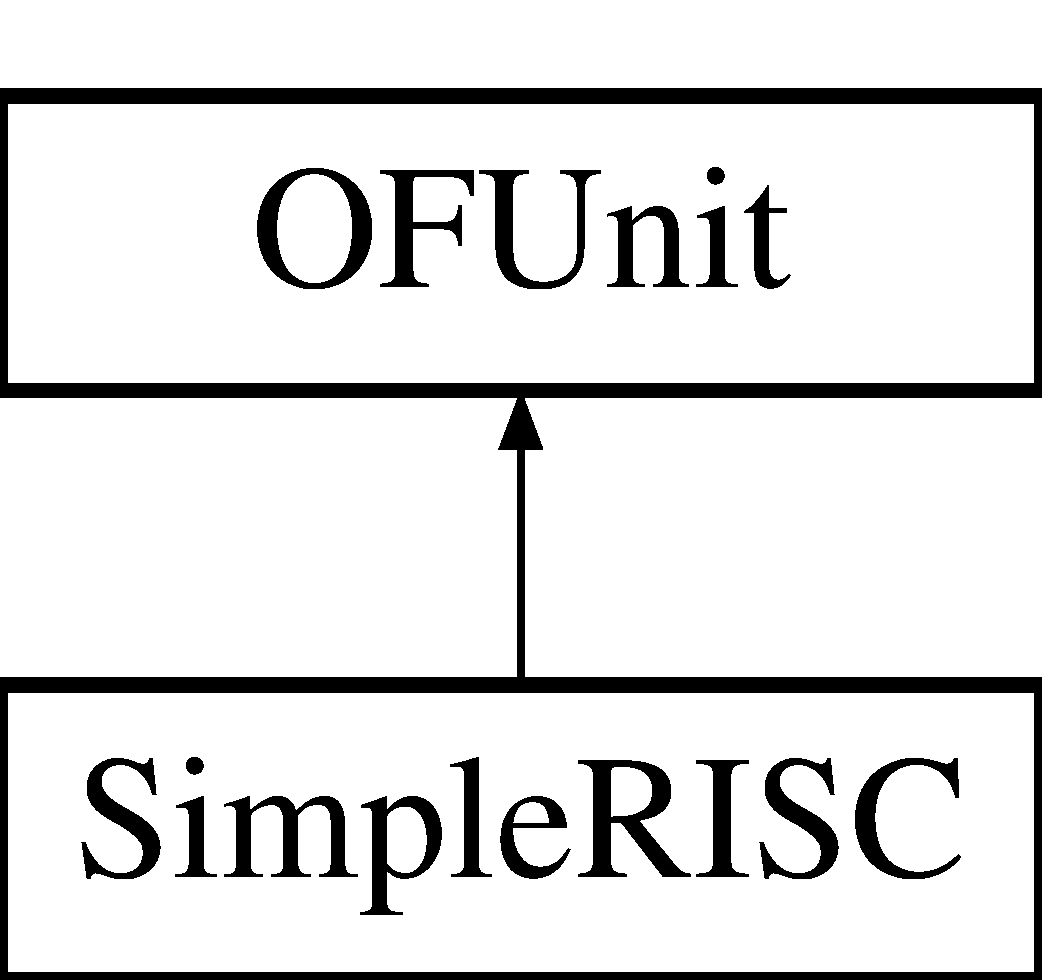
\includegraphics[height=2.000000cm]{class_o_f_unit}
\end{center}
\end{figure}
\subsection*{Entities}
\begin{DoxyCompactItemize}
\item 
\hyperlink{class_o_f_unit_1_1_o_f_u}{O\-F\-U} architecture
\begin{DoxyCompactList}\small\item\em \hyperlink{class_o_f_unit_1_1_o_f_u}{O\-F\-U} is the architectural description of the operand fetch unit and register file. \end{DoxyCompactList}\end{DoxyCompactItemize}
\subsection*{Libraries}
 \begin{DoxyCompactItemize}
\item 
\hypertarget{class_o_f_unit_a0a6af6eef40212dbaf130d57ce711256}{\hyperlink{class_o_f_unit_a0a6af6eef40212dbaf130d57ce711256}{ieee} }\label{class_o_f_unit_a0a6af6eef40212dbaf130d57ce711256}

\end{DoxyCompactItemize}
\subsection*{Use Clauses}
 \begin{DoxyCompactItemize}
\item 
\hypertarget{class_o_f_unit_a43ecb358105806229eb7a3074fc4d577}{\hyperlink{class_o_f_unit_a43ecb358105806229eb7a3074fc4d577}{ieee.\-std\-\_\-logic\-\_\-1164.\-all}   }\label{class_o_f_unit_a43ecb358105806229eb7a3074fc4d577}

\item 
\hypertarget{class_o_f_unit_a631689596594b2068e0ee8dadd0931fe}{\hyperlink{class_o_f_unit_a631689596594b2068e0ee8dadd0931fe}{ieee.\-numeric\-\_\-std.\-all}   }\label{class_o_f_unit_a631689596594b2068e0ee8dadd0931fe}

\end{DoxyCompactItemize}
\subsection*{Ports}
 \begin{DoxyCompactItemize}
\item 
\hypertarget{class_o_f_unit_a94f6b72ef22091aa46807c9d89632a9b}{\hyperlink{class_o_f_unit_a94f6b72ef22091aa46807c9d89632a9b}{clk}  {\bfseries {\bfseries \textcolor{vhdlkeyword}{in}\textcolor{vhdlchar}{ }}} {\bfseries \textcolor{comment}{std\-\_\-logic}\textcolor{vhdlchar}{ }} }\label{class_o_f_unit_a94f6b72ef22091aa46807c9d89632a9b}

\begin{DoxyCompactList}\small\item\em C\-L\-O\-C\-K for the unit. \end{DoxyCompactList}\item 
\hypertarget{class_o_f_unit_a187326d2b4b17c46dcaeead2064c8c82}{\hyperlink{class_o_f_unit_a187326d2b4b17c46dcaeead2064c8c82}{Instruction}  {\bfseries {\bfseries \textcolor{vhdlkeyword}{in}\textcolor{vhdlchar}{ }}} {\bfseries \textcolor{comment}{std\-\_\-logic\-\_\-vector}\textcolor{vhdlchar}{ }\textcolor{vhdlchar}{(}\textcolor{vhdlchar}{ } \textcolor{vhdldigit}{31} \textcolor{vhdlchar}{ }\textcolor{vhdlchar}{ }\textcolor{vhdlchar}{ }\textcolor{vhdlkeyword}{downto}\textcolor{vhdlchar}{ }\textcolor{vhdlchar}{ }\textcolor{vhdlchar}{ } \textcolor{vhdldigit}{0} \textcolor{vhdlchar}{ }\textcolor{vhdlchar}{)}\textcolor{vhdlchar}{ }} }\label{class_o_f_unit_a187326d2b4b17c46dcaeead2064c8c82}

\begin{DoxyCompactList}\small\item\em Complete 32 bit instruction code. \end{DoxyCompactList}\item 
\hypertarget{class_o_f_unit_a15b73a10b7d4cf16cdae7729404b05da}{\hyperlink{class_o_f_unit_a15b73a10b7d4cf16cdae7729404b05da}{P\-C}  {\bfseries {\bfseries \textcolor{vhdlkeyword}{in}\textcolor{vhdlchar}{ }}} {\bfseries \textcolor{comment}{std\-\_\-logic\-\_\-vector}\textcolor{vhdlchar}{ }\textcolor{vhdlchar}{(}\textcolor{vhdlchar}{ } \textcolor{vhdldigit}{31} \textcolor{vhdlchar}{ }\textcolor{vhdlchar}{ }\textcolor{vhdlchar}{ }\textcolor{vhdlkeyword}{downto}\textcolor{vhdlchar}{ }\textcolor{vhdlchar}{ }\textcolor{vhdlchar}{ } \textcolor{vhdldigit}{0} \textcolor{vhdlchar}{ }\textcolor{vhdlchar}{)}\textcolor{vhdlchar}{ }} }\label{class_o_f_unit_a15b73a10b7d4cf16cdae7729404b05da}

\begin{DoxyCompactList}\small\item\em Program Counter. \end{DoxyCompactList}\item 
\hypertarget{class_o_f_unit_a15f3af98c390c64fec95e54717345647}{\hyperlink{class_o_f_unit_a15f3af98c390c64fec95e54717345647}{alu\-R}  {\bfseries {\bfseries \textcolor{vhdlkeyword}{in}\textcolor{vhdlchar}{ }}} {\bfseries \textcolor{comment}{std\-\_\-logic\-\_\-vector}\textcolor{vhdlchar}{ }\textcolor{vhdlchar}{(}\textcolor{vhdlchar}{ } \textcolor{vhdldigit}{31} \textcolor{vhdlchar}{ }\textcolor{vhdlchar}{ }\textcolor{vhdlchar}{ }\textcolor{vhdlkeyword}{downto}\textcolor{vhdlchar}{ }\textcolor{vhdlchar}{ }\textcolor{vhdlchar}{ } \textcolor{vhdldigit}{0} \textcolor{vhdlchar}{ }\textcolor{vhdlchar}{)}\textcolor{vhdlchar}{ }} }\label{class_o_f_unit_a15f3af98c390c64fec95e54717345647}

\begin{DoxyCompactList}\small\item\em A\-L\-U Result that is to be written in register in case of an alu instrcution. \end{DoxyCompactList}\item 
\hypertarget{class_o_f_unit_a853c1b450b6ba2b91af02d5fdb93bc32}{\hyperlink{class_o_f_unit_a853c1b450b6ba2b91af02d5fdb93bc32}{ld\-R}  {\bfseries {\bfseries \textcolor{vhdlkeyword}{in}\textcolor{vhdlchar}{ }}} {\bfseries \textcolor{comment}{std\-\_\-logic\-\_\-vector}\textcolor{vhdlchar}{ }\textcolor{vhdlchar}{(}\textcolor{vhdlchar}{ } \textcolor{vhdldigit}{31} \textcolor{vhdlchar}{ }\textcolor{vhdlchar}{ }\textcolor{vhdlchar}{ }\textcolor{vhdlkeyword}{downto}\textcolor{vhdlchar}{ }\textcolor{vhdlchar}{ }\textcolor{vhdlchar}{ } \textcolor{vhdldigit}{0} \textcolor{vhdlchar}{ }\textcolor{vhdlchar}{)}\textcolor{vhdlchar}{ }} }\label{class_o_f_unit_a853c1b450b6ba2b91af02d5fdb93bc32}

\begin{DoxyCompactList}\small\item\em Load Result that is to be written in register in case of a load instrcution. \end{DoxyCompactList}\item 
\hypertarget{class_o_f_unit_ada232e9bb13e48ba67c49897a8f2a98c}{\hyperlink{class_o_f_unit_ada232e9bb13e48ba67c49897a8f2a98c}{is\-St}  {\bfseries {\bfseries \textcolor{vhdlkeyword}{in}\textcolor{vhdlchar}{ }}} {\bfseries \textcolor{comment}{boolean}\textcolor{vhdlchar}{ }} }\label{class_o_f_unit_ada232e9bb13e48ba67c49897a8f2a98c}

\begin{DoxyCompactList}\small\item\em boolean for store instruction \end{DoxyCompactList}\item 
\hypertarget{class_o_f_unit_a4f328a19e16850a109722d3bf847ea76}{\hyperlink{class_o_f_unit_a4f328a19e16850a109722d3bf847ea76}{is\-Ld}  {\bfseries {\bfseries \textcolor{vhdlkeyword}{in}\textcolor{vhdlchar}{ }}} {\bfseries \textcolor{comment}{boolean}\textcolor{vhdlchar}{ }} }\label{class_o_f_unit_a4f328a19e16850a109722d3bf847ea76}

\begin{DoxyCompactList}\small\item\em boolean for load instruction \end{DoxyCompactList}\item 
\hypertarget{class_o_f_unit_a2824764974bcc836bcb65f7660df3501}{\hyperlink{class_o_f_unit_a2824764974bcc836bcb65f7660df3501}{is\-Wb}  {\bfseries {\bfseries \textcolor{vhdlkeyword}{in}\textcolor{vhdlchar}{ }}} {\bfseries \textcolor{comment}{boolean}\textcolor{vhdlchar}{ }} }\label{class_o_f_unit_a2824764974bcc836bcb65f7660df3501}

\begin{DoxyCompactList}\small\item\em boolean for writeback that is its true when something is to be written in the register file \end{DoxyCompactList}\item 
\hypertarget{class_o_f_unit_acc9e88547584f5ec26824185166a68ec}{\hyperlink{class_o_f_unit_acc9e88547584f5ec26824185166a68ec}{is\-Ret}  {\bfseries {\bfseries \textcolor{vhdlkeyword}{in}\textcolor{vhdlchar}{ }}} {\bfseries \textcolor{comment}{boolean}\textcolor{vhdlchar}{ }} }\label{class_o_f_unit_acc9e88547584f5ec26824185166a68ec}

\begin{DoxyCompactList}\small\item\em boolean which states whether the instruction is 'ret' \end{DoxyCompactList}\item 
\hypertarget{class_o_f_unit_a7c4ebeb76d12c2b065431834e3e40b61}{\hyperlink{class_o_f_unit_a7c4ebeb76d12c2b065431834e3e40b61}{is\-Call}  {\bfseries {\bfseries \textcolor{vhdlkeyword}{in}\textcolor{vhdlchar}{ }}} {\bfseries \textcolor{comment}{boolean}\textcolor{vhdlchar}{ }} }\label{class_o_f_unit_a7c4ebeb76d12c2b065431834e3e40b61}

\begin{DoxyCompactList}\small\item\em boolean which states whether the instruction is 'call' \end{DoxyCompactList}\item 
\hypertarget{class_o_f_unit_ad63c399e5906690f784966193e1f33f1}{\hyperlink{class_o_f_unit_ad63c399e5906690f784966193e1f33f1}{immediate}  {\bfseries {\bfseries \textcolor{vhdlkeyword}{out}\textcolor{vhdlchar}{ }}} {\bfseries \textcolor{comment}{std\-\_\-logic\-\_\-vector}\textcolor{vhdlchar}{ }\textcolor{vhdlchar}{(}\textcolor{vhdlchar}{ } \textcolor{vhdldigit}{31} \textcolor{vhdlchar}{ }\textcolor{vhdlchar}{ }\textcolor{vhdlchar}{ }\textcolor{vhdlkeyword}{downto}\textcolor{vhdlchar}{ }\textcolor{vhdlchar}{ }\textcolor{vhdlchar}{ } \textcolor{vhdldigit}{0} \textcolor{vhdlchar}{ }\textcolor{vhdlchar}{)}\textcolor{vhdlchar}{ }} }\label{class_o_f_unit_ad63c399e5906690f784966193e1f33f1}

\begin{DoxyCompactList}\small\item\em 32 bit immediate that has to be computed \end{DoxyCompactList}\item 
\hypertarget{class_o_f_unit_a0d338d7f0493ce29501b3eb557de0a67}{\hyperlink{class_o_f_unit_a0d338d7f0493ce29501b3eb557de0a67}{branch\-Target}  {\bfseries {\bfseries \textcolor{vhdlkeyword}{out}\textcolor{vhdlchar}{ }}} {\bfseries \textcolor{comment}{std\-\_\-logic\-\_\-vector}\textcolor{vhdlchar}{ }\textcolor{vhdlchar}{(}\textcolor{vhdlchar}{ } \textcolor{vhdldigit}{31} \textcolor{vhdlchar}{ }\textcolor{vhdlchar}{ }\textcolor{vhdlchar}{ }\textcolor{vhdlkeyword}{downto}\textcolor{vhdlchar}{ }\textcolor{vhdlchar}{ }\textcolor{vhdlchar}{ } \textcolor{vhdldigit}{0} \textcolor{vhdlchar}{ }\textcolor{vhdlchar}{)}\textcolor{vhdlchar}{ }} }\label{class_o_f_unit_a0d338d7f0493ce29501b3eb557de0a67}

\begin{DoxyCompactList}\small\item\em This is the branch target which is used in case of a branch or call instruction. \end{DoxyCompactList}\item 
\hypertarget{class_o_f_unit_a923e4330bf1a7966baa0589fb6b397e6}{\hyperlink{class_o_f_unit_a923e4330bf1a7966baa0589fb6b397e6}{op1}  {\bfseries {\bfseries \textcolor{vhdlkeyword}{out}\textcolor{vhdlchar}{ }}} {\bfseries \textcolor{comment}{std\-\_\-logic\-\_\-vector}\textcolor{vhdlchar}{ }\textcolor{vhdlchar}{(}\textcolor{vhdlchar}{ } \textcolor{vhdldigit}{31} \textcolor{vhdlchar}{ }\textcolor{vhdlchar}{ }\textcolor{vhdlchar}{ }\textcolor{vhdlkeyword}{downto}\textcolor{vhdlchar}{ }\textcolor{vhdlchar}{ }\textcolor{vhdlchar}{ } \textcolor{vhdldigit}{0} \textcolor{vhdlchar}{ }\textcolor{vhdlchar}{)}\textcolor{vhdlchar}{ }} }\label{class_o_f_unit_a923e4330bf1a7966baa0589fb6b397e6}

\begin{DoxyCompactList}\small\item\em First pperand. \end{DoxyCompactList}\item 
\hypertarget{class_o_f_unit_a014e99b0b5a371c08961e8a6b658d3f4}{\hyperlink{class_o_f_unit_a014e99b0b5a371c08961e8a6b658d3f4}{op2}  {\bfseries {\bfseries \textcolor{vhdlkeyword}{out}\textcolor{vhdlchar}{ }}} {\bfseries \textcolor{comment}{std\-\_\-logic\-\_\-vector}\textcolor{vhdlchar}{ }\textcolor{vhdlchar}{(}\textcolor{vhdlchar}{ } \textcolor{vhdldigit}{31} \textcolor{vhdlchar}{ }\textcolor{vhdlchar}{ }\textcolor{vhdlchar}{ }\textcolor{vhdlkeyword}{downto}\textcolor{vhdlchar}{ }\textcolor{vhdlchar}{ }\textcolor{vhdlchar}{ } \textcolor{vhdldigit}{0} \textcolor{vhdlchar}{ }\textcolor{vhdlchar}{)}\textcolor{vhdlchar}{ }} }\label{class_o_f_unit_a014e99b0b5a371c08961e8a6b658d3f4}

\begin{DoxyCompactList}\small\item\em Second Operand. \end{DoxyCompactList}\end{DoxyCompactItemize}


\subsection{Detailed Description}
This the Operand Fetch Unit which also contains the register file implementation. 

The documentation for this class was generated from the following file\-:\begin{DoxyCompactItemize}
\item 
\hyperlink{_o_f_unit_8vhdl}{O\-F\-Unit.\-vhdl}\end{DoxyCompactItemize}

\hypertarget{class_simple_r_i_s_c}{\section{Simple\-R\-I\-S\-C Entity Reference}
\label{class_simple_r_i_s_c}\index{Simple\-R\-I\-S\-C@{Simple\-R\-I\-S\-C}}
}


This is empty shell for the main compilation of all the other components in the processor.  


Inheritance diagram for Simple\-R\-I\-S\-C\-:\begin{figure}[H]
\begin{center}
\leavevmode
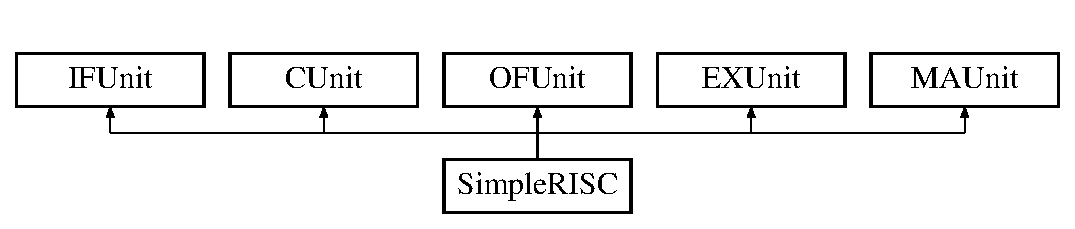
\includegraphics[height=2.000000cm]{class_simple_r_i_s_c}
\end{center}
\end{figure}
\subsection*{Entities}
\begin{DoxyCompactItemize}
\item 
\hyperlink{class_simple_r_i_s_c_1_1main}{main} architecture
\end{DoxyCompactItemize}
\subsection*{Libraries}
 \begin{DoxyCompactItemize}
\item 
\hypertarget{class_simple_r_i_s_c_a0a6af6eef40212dbaf130d57ce711256}{\hyperlink{class_simple_r_i_s_c_a0a6af6eef40212dbaf130d57ce711256}{ieee} }\label{class_simple_r_i_s_c_a0a6af6eef40212dbaf130d57ce711256}

\end{DoxyCompactItemize}
\subsection*{Use Clauses}
 \begin{DoxyCompactItemize}
\item 
\hypertarget{class_simple_r_i_s_c_a43ecb358105806229eb7a3074fc4d577}{\hyperlink{class_simple_r_i_s_c_a43ecb358105806229eb7a3074fc4d577}{ieee.\-std\-\_\-logic\-\_\-1164.\-all}   }\label{class_simple_r_i_s_c_a43ecb358105806229eb7a3074fc4d577}

\item 
\hypertarget{class_simple_r_i_s_c_a631689596594b2068e0ee8dadd0931fe}{\hyperlink{class_simple_r_i_s_c_a631689596594b2068e0ee8dadd0931fe}{ieee.\-numeric\-\_\-std.\-all}   }\label{class_simple_r_i_s_c_a631689596594b2068e0ee8dadd0931fe}

\end{DoxyCompactItemize}


\subsection{Detailed Description}
This is empty shell for the main compilation of all the other components in the processor. 

The documentation for this class was generated from the following file\-:\begin{DoxyCompactItemize}
\item 
\hyperlink{_simple_r_i_s_c_8vhdl}{Simple\-R\-I\-S\-C.\-vhdl}\end{DoxyCompactItemize}

\chapter{File Documentation}
\hypertarget{_c_unit_8vhdl}{\section{C\-Unit.\-vhdl File Reference}
\label{_c_unit_8vhdl}\index{C\-Unit.\-vhdl@{C\-Unit.\-vhdl}}
}


This file for the implementation of a Control Unit for the processor.  


\subsection*{Entities}
\begin{DoxyCompactItemize}
\item 
\hyperlink{class_c_unit}{C\-Unit} entity
\begin{DoxyCompactList}\small\item\em This is the unit that generates the control signals. \end{DoxyCompactList}\item 
\hyperlink{class_c_unit_1_1_c_u}{C\-U} architecture
\begin{DoxyCompactList}\small\item\em \hyperlink{class_c_unit_1_1_c_u}{C\-U} is the architectural description of the Control Unit. \end{DoxyCompactList}\end{DoxyCompactItemize}


\subsection{Detailed Description}
This file for the implementation of a Control Unit for the processor. \begin{DoxyAuthor}{Author}
Kunal Singhal and Swapnil Palash 
\end{DoxyAuthor}

\hypertarget{_e_x_unit_8vhdl}{\section{E\-X\-Unit.\-vhdl File Reference}
\label{_e_x_unit_8vhdl}\index{E\-X\-Unit.\-vhdl@{E\-X\-Unit.\-vhdl}}
}


This file is for the Arithmetic and logic Unit of the processor.  


\subsection*{Entities}
\begin{DoxyCompactItemize}
\item 
\hyperlink{class_e_x_unit}{E\-X\-Unit} entity
\begin{DoxyCompactList}\small\item\em This is the unit that implements the A\-L\-U and branch Unit. \end{DoxyCompactList}\item 
\hyperlink{class_e_x_unit_1_1_a_l_u___b_u}{A\-L\-U\-\_\-\-B\-U} architecture
\begin{DoxyCompactList}\small\item\em O\-F\-U is the architectural description of the E\-X Unit. \end{DoxyCompactList}\end{DoxyCompactItemize}


\subsection{Detailed Description}
This file is for the Arithmetic and logic Unit of the processor. \begin{DoxyAuthor}{Author}
Kunal Singhal and Swapnil Palash 
\end{DoxyAuthor}

\hypertarget{file_read_8vhdl}{\section{file\-Read.\-vhdl File Reference}
\label{file_read_8vhdl}\index{file\-Read.\-vhdl@{file\-Read.\-vhdl}}
}


This file for the implementation of file reading function.  


\subsection*{Entities}
\begin{DoxyCompactItemize}
\item 
\hyperlink{classfile_read}{file\-Read} package
\begin{DoxyCompactList}\small\item\em This function converts a char to std\-\_\-logic. \end{DoxyCompactList}\item 
\hyperlink{class__file_read}{file\-Read} package body
\end{DoxyCompactItemize}


\subsection{Detailed Description}
This file for the implementation of file reading function. \begin{DoxyAuthor}{Author}
Kunal Singhal and Swapnil Palash 
\end{DoxyAuthor}

\hypertarget{_i_f_unit_8vhdl}{\section{I\-F\-Unit.\-vhdl File Reference}
\label{_i_f_unit_8vhdl}\index{I\-F\-Unit.\-vhdl@{I\-F\-Unit.\-vhdl}}
}


This file for the implementation of a Instruction Fetch Unit for the processor.  


\subsection*{Entities}
\begin{DoxyCompactItemize}
\item 
\hyperlink{class_i_f_unit}{I\-F\-Unit} entity
\begin{DoxyCompactList}\small\item\em This is the unit that implements the Instruction fetch Unit. \end{DoxyCompactList}\item 
\hyperlink{class_i_f_unit_1_1_i_m}{I\-M} architecture
\begin{DoxyCompactList}\small\item\em \hyperlink{class_i_f_unit_1_1_i_m}{I\-M} is the architectural description of the Instruction Fetch Unit. \end{DoxyCompactList}\end{DoxyCompactItemize}


\subsection{Detailed Description}
This file for the implementation of a Instruction Fetch Unit for the processor. \begin{DoxyAuthor}{Author}
Kunal Singhal and Swapnil Palash 
\end{DoxyAuthor}

\hypertarget{_m_a_unit_8vhdl}{\section{M\-A\-Unit.\-vhdl File Reference}
\label{_m_a_unit_8vhdl}\index{M\-A\-Unit.\-vhdl@{M\-A\-Unit.\-vhdl}}
}


This file for the implementation of a memory for the processor.  


\subsection*{Entities}
\begin{DoxyCompactItemize}
\item 
\hyperlink{class_m_a_unit}{M\-A\-Unit} entity
\begin{DoxyCompactList}\small\item\em This is the unit that implements a R\-A\-M. \end{DoxyCompactList}\item 
\hyperlink{class_m_a_unit_1_1_d_m}{D\-M} architecture
\begin{DoxyCompactList}\small\item\em \hyperlink{class_m_a_unit_1_1_d_m}{D\-M} is the architecture of the Memory Unit. \end{DoxyCompactList}\end{DoxyCompactItemize}


\subsection{Detailed Description}
This file for the implementation of a memory for the processor. \begin{DoxyAuthor}{Author}
Kunal Singhal and Swapnil Palash 
\end{DoxyAuthor}

\hypertarget{_o_f_unit_8vhdl}{\section{O\-F\-Unit.\-vhdl File Reference}
\label{_o_f_unit_8vhdl}\index{O\-F\-Unit.\-vhdl@{O\-F\-Unit.\-vhdl}}
}


Operand Fetch unit as well as register read and write operations implemented.  


\subsection*{Entities}
\begin{DoxyCompactItemize}
\item 
\hyperlink{class_o_f_unit}{O\-F\-Unit} entity
\begin{DoxyCompactList}\small\item\em This the Operand Fetch Unit which also contains the register file implementation. \end{DoxyCompactList}\item 
\hyperlink{class_o_f_unit_1_1_o_f_u}{O\-F\-U} architecture
\begin{DoxyCompactList}\small\item\em \hyperlink{class_o_f_unit_1_1_o_f_u}{O\-F\-U} is the architectural description of the operand fetch unit and register file. \end{DoxyCompactList}\end{DoxyCompactItemize}


\subsection{Detailed Description}
Operand Fetch unit as well as register read and write operations implemented. \begin{DoxyAuthor}{Author}
Kunal Singhal and Swapnil Palash 
\end{DoxyAuthor}

\hypertarget{_simple_r_i_s_c_8vhdl}{\section{Simple\-R\-I\-S\-C.\-vhdl File Reference}
\label{_simple_r_i_s_c_8vhdl}\index{Simple\-R\-I\-S\-C.\-vhdl@{Simple\-R\-I\-S\-C.\-vhdl}}
}


This is compilation of all the components of the processor.  


\subsection*{Entities}
\begin{DoxyCompactItemize}
\item 
\hyperlink{class_simple_r_i_s_c}{Simple\-R\-I\-S\-C} entity
\begin{DoxyCompactList}\small\item\em This is empty shell for the main compilation of all the other components in the processor. \end{DoxyCompactList}\item 
\hyperlink{class_simple_r_i_s_c_1_1main}{main} architecture
\end{DoxyCompactItemize}


\subsection{Detailed Description}
This is compilation of all the components of the processor. \begin{DoxyAuthor}{Author}
Kunal Singhal and Swapnil Palash 
\end{DoxyAuthor}

%--- End generated contents ---

% Index
\newpage
\phantomsection
\addcontentsline{toc}{chapter}{Index}
\printindex

\end{document}
